% Generated fragments require trusted human review before compilation.
% This binder never requests shell escape or runs external tools.
\documentclass[11pt]{article}
% Trusted shared apparatus. Requires LuaLaTeX; never use shell escape.
\usepackage{fontspec}
\defaultfontfeatures{Ligatures=TeX}
\IfFontExistsTF{Noto Serif}{\setmainfont{Noto Serif}}{%
  \IfFontExistsTF{DejaVu Serif}{\setmainfont{DejaVu Serif}}{%
    \IfFontExistsTF{Times New Roman}{\setmainfont{Times New Roman}}{%
      \PackageError{gelfand-binder}{No configured Cyrillic serif font installed}{Install Noto Serif or DejaVu Serif, or select an installed Cyrillic font.}%
    }%
  }%
}
\IfFontExistsTF{Noto Sans}{\setsansfont{Noto Sans}}{%
  \IfFontExistsTF{DejaVu Sans}{\setsansfont{DejaVu Sans}}{\setsansfont{Arial}}%
}
\IfFontExistsTF{Noto Sans Mono}{\setmonofont{Noto Sans Mono}}{%
  \IfFontExistsTF{DejaVu Sans Mono}{\setmonofont{DejaVu Sans Mono}}{\setmonofont{Courier New}}%
}
\usepackage[a4paper,margin=22mm]{geometry}
\usepackage{amsmath,amssymb,amsthm,mathtools}
\usepackage{xcolor}
\usepackage{tikz}
\usepackage{tikz-cd}
\usetikzlibrary{arrows.meta,positioning,calc}
\usepackage{hyperref}
\hypersetup{unicode=true,colorlinks=true,linkcolor=blue,pdftitle={Gelfand transcription binder}}
\newtheorem{theorem}{Theorem}
\newtheorem{lemma}{Lemma}
\newtheorem{proposition}{Proposition}
\newtheorem{corollary}{Corollary}
\theoremstyle{definition}
\newtheorem{definition}{Definition}
\newtheorem{example}{Example}
\theoremstyle{remark}
\newtheorem{remark}{Remark}
\setlength{\parindent}{0pt}
\setlength{\parskip}{0.55em}
\setlength{\emergencystretch}{3em}
\newcommand{\SourcePage}[2]{%
  \clearpage\phantomsection\label{#1:source-page}%
  \addcontentsline{toc}{subsection}{#1}%
  {\small\sffamily\color{blue!60!black}Source scan frame: #1; visible page/leaf label: #2}\par\medskip%
}
\newcommand{\Unclear}[3]{%
  \begingroup\color{orange!70!black}%
  [Unresolved reading #1/#2: #3]\endgroup%
}
\newcommand{\Incomplete}[3]{%
  \par\begingroup\color{red!65!black}\textbf{Incomplete #1/#2:} #3\endgroup\par%
}
\newcommand{\SourceFigure}[3]{%
  \par\begingroup\color{blue!60!black}\textbf{\hyperref[#1:source-page]{Source figure #1/#2}:} #3%
  \par\textit{Consult the authoritative scan at this locator.}\endgroup\par%
}



% Reader layout only. Original diplomatic text is retained verbatim.
\setlength{\parskip}{0.35em}
\setlength{\emergencystretch}{4em}
\renewcommand{\SourcePage}[2]{%
  \par\addvspace{1em}\phantomsection\label{#1:source-page}%
  \addcontentsline{toc}{subsection}{#1}%
  {\footnotesize\sffamily\color{blue!55!black}#1%
    \def\givenlabel{#2}\def\nolabel{unlabelled}%
    \ifx\givenlabel\nolabel\else\quad[номер в источнике: #2]\fi
  }\par\nobreak\smallskip%
}
\renewcommand{\Unclear}[3]{%
  \begingroup\color{orange!65!black}%
  \ifmmode\text{[неясно: #3]}\else[неясно: #3]\fi\endgroup%
}
\renewcommand{\Incomplete}[3]{%
  \par\begingroup\color{red!60!black}\textbf{Неразобранный фрагмент:} #3%
  \endgroup\par%
}
\renewcommand{\SourceFigure}[3]{%
  \par\begingroup\color{blue!55!black}\textbf{Рисунок:} #3%
  \par{\small\textit{Исходный рисунок: \hyperref[#1:source-page]{#1}, #2.}}%
  \endgroup\par%
}
\hypersetup{pdftitle={Семинар И. М. Гельфанда. Дипломатическая транскрипция},pdfauthor={},pdfsubject={Русское рабочее издание с отмеченными сомнительными чтениями}}

\usepackage[normalem]{ulem}
\usepackage{newunicodechar}
\usepackage{adjustbox}
\newfontfamily\SourceSymbolFont{Segoe UI Symbol}
\newfontfamily\SourceCJKFont{MS Gothic}
\let\DiplomaticMathUnderline\underline
\renewcommand{\underline}[1]{\ifmmode\DiplomaticMathUnderline{#1}\else\uline{#1}\fi}
\newunicodechar{→}{\ifmmode\text{{\SourceSymbolFont\char"2192}}\else{\SourceSymbolFont\char"2192}\fi}
\newunicodechar{⇒}{\ifmmode\text{{\SourceSymbolFont\char"21D2}}\else{\SourceSymbolFont\char"21D2}\fi}
\newunicodechar{∀}{\ifmmode\text{{\SourceSymbolFont\char"2200}}\else{\SourceSymbolFont\char"2200}\fi}
\newunicodechar{∂}{\ifmmode\text{{\SourceSymbolFont\char"2202}}\else{\SourceSymbolFont\char"2202}\fi}
\newunicodechar{∈}{\ifmmode\text{{\SourceSymbolFont\char"2208}}\else{\SourceSymbolFont\char"2208}\fi}
\newunicodechar{∌}{\ifmmode\text{{\SourceSymbolFont\char"220C}}\else{\SourceSymbolFont\char"220C}\fi}
\newunicodechar{√}{\ifmmode\text{{\SourceSymbolFont\char"221A}}\else{\SourceSymbolFont\char"221A}\fi}
\newunicodechar{∞}{\ifmmode\text{{\SourceSymbolFont\char"221E}}\else{\SourceSymbolFont\char"221E}\fi}
\newunicodechar{∧}{\ifmmode\text{{\SourceSymbolFont\char"2227}}\else{\SourceSymbolFont\char"2227}\fi}
\newunicodechar{∩}{\ifmmode\text{{\SourceSymbolFont\char"2229}}\else{\SourceSymbolFont\char"2229}\fi}
\newunicodechar{∪}{\ifmmode\text{{\SourceSymbolFont\char"222A}}\else{\SourceSymbolFont\char"222A}\fi}
\newunicodechar{∫}{\ifmmode\text{{\SourceSymbolFont\char"222B}}\else{\SourceSymbolFont\char"222B}\fi}
\newunicodechar{∴}{\ifmmode\text{{\SourceSymbolFont\char"2234}}\else{\SourceSymbolFont\char"2234}\fi}
\newunicodechar{∼}{\ifmmode\text{{\SourceSymbolFont\char"223C}}\else{\SourceSymbolFont\char"223C}\fi}
\newunicodechar{≈}{\ifmmode\text{{\SourceSymbolFont\char"2248}}\else{\SourceSymbolFont\char"2248}\fi}
\newunicodechar{≠}{\ifmmode\text{{\SourceSymbolFont\char"2260}}\else{\SourceSymbolFont\char"2260}\fi}
\newunicodechar{≤}{\ifmmode\text{{\SourceSymbolFont\char"2264}}\else{\SourceSymbolFont\char"2264}\fi}
\newunicodechar{≥}{\ifmmode\text{{\SourceSymbolFont\char"2265}}\else{\SourceSymbolFont\char"2265}\fi}
\newunicodechar{⊕}{\ifmmode\text{{\SourceSymbolFont\char"2295}}\else{\SourceSymbolFont\char"2295}\fi}
\newunicodechar{⊗}{\ifmmode\text{{\SourceSymbolFont\char"2297}}\else{\SourceSymbolFont\char"2297}\fi}
\newunicodechar{①}{\ifmmode\text{{\SourceSymbolFont\char"2460}}\else{\SourceSymbolFont\char"2460}\fi}
\newunicodechar{②}{\ifmmode\text{{\SourceSymbolFont\char"2461}}\else{\SourceSymbolFont\char"2461}\fi}
\newunicodechar{③}{\ifmmode\text{{\SourceSymbolFont\char"2462}}\else{\SourceSymbolFont\char"2462}\fi}
\newunicodechar{④}{\ifmmode\text{{\SourceSymbolFont\char"2463}}\else{\SourceSymbolFont\char"2463}\fi}
\newunicodechar{Ⓗ}{\ifmmode\text{{\SourceSymbolFont\char"24BD}}\else{\SourceSymbolFont\char"24BD}\fi}
\newunicodechar{〃}{\ifmmode\text{{\SourceCJKFont\char"3003}}\else{\SourceCJKFont\char"3003}\fi}


% Reader revision 3. Annotation wording and candidates remain unchanged.
\setmainfont{NotoSerif-Regular.ttf}[Path=C:/Windows/Fonts/,ItalicFont=NotoSerif-Italic.ttf,BoldFont=NotoSerif-Bold.ttf,BoldItalicFont=NotoSerif-BoldItalic.ttf]
\usetikzlibrary{shapes.geometric,decorations.pathreplacing,decorations.markings,patterns,fit}
\newsavebox{\ReaderAnnotationBox}
\newcommand{\ReaderAnnotation}[1]{%
  \sbox{\ReaderAnnotationBox}{[неясно: #1]}%
  \ifdim\wd\ReaderAnnotationBox>.70\linewidth
    \parbox[t]{.70\linewidth}{\raggedright[неясно: #1]}%
  \else\usebox{\ReaderAnnotationBox}\fi%
}
\ExplSyntaxOn
\cs_new_protected:Npn \reader_unclear_candidate:n #1
 {
  \tl_set:Nx \l_tmpa_tl { \tl_to_str:n {#1} }
  % Text explicitly guarded inside a mathematical candidate remains math-safe.
  \regex_replace_all:nnN { \\(?:text|textrm|textnormal|textbf|operatorname)\s*\{[^{}]*\} } { } \l_tmpa_tl
  \regex_match:nVTF { [\x{0400}-\x{052F}] | \$ } \l_tmpa_tl
   { \ifmmode \text{\ReaderAnnotation{#1}} \else \ReaderAnnotation{#1} \fi }
   {
    \ifmmode
      [\text{неясно:~}#1]
    \else
      \regex_match:nVTF { [_^] | \\ } \l_tmpa_tl
       { \ensuremath{[\text{неясно:~}#1]} }
       { \ReaderAnnotation{#1} }
    \fi
   }
 }
\RenewDocumentCommand \Unclear { m m m }
 { \begingroup\color{orange!65!black}\reader_unclear_candidate:n{#3}\endgroup }
\ExplSyntaxOff
\newsavebox{\ReaderIncompleteBox}
\newcommand{\ReaderIncompleteNote}[1]{%
 \sbox{\ReaderIncompleteBox}{\textbf{Неразобранный фрагмент:} #1}%
 \ifdim\wd\ReaderIncompleteBox>.70\linewidth
  \parbox[t]{.70\linewidth}{\raggedright\textbf{Неразобранный фрагмент:} #1}%
 \else\usebox{\ReaderIncompleteBox}\fi%
}
\renewcommand{\Incomplete}[3]{%
 \ifmmode\text{\color{red!60!black}\ReaderIncompleteNote{#3}}%
 \else\leavevmode\begingroup\color{red!60!black}\ReaderIncompleteNote{#3}\endgroup\fi%
}
% Ragged right avoids stretching long untranslated abbreviations into margins.
\AtBeginDocument{\raggedright}
\newunicodechar{А}{\ifmmode\text{\char"410\relax}\else\char"410\relax\fi}
\newunicodechar{Б}{\ifmmode\text{\char"411\relax}\else\char"411\relax\fi}
\newunicodechar{В}{\ifmmode\text{\char"412\relax}\else\char"412\relax\fi}
\newunicodechar{Г}{\ifmmode\text{\char"413\relax}\else\char"413\relax\fi}
\newunicodechar{Д}{\ifmmode\text{\char"414\relax}\else\char"414\relax\fi}
\newunicodechar{Е}{\ifmmode\text{\char"415\relax}\else\char"415\relax\fi}
\newunicodechar{Ж}{\ifmmode\text{\char"416\relax}\else\char"416\relax\fi}
\newunicodechar{З}{\ifmmode\text{\char"417\relax}\else\char"417\relax\fi}
\newunicodechar{И}{\ifmmode\text{\char"418\relax}\else\char"418\relax\fi}
\newunicodechar{Й}{\ifmmode\text{\char"419\relax}\else\char"419\relax\fi}
\newunicodechar{К}{\ifmmode\text{\char"41A\relax}\else\char"41A\relax\fi}
\newunicodechar{Л}{\ifmmode\text{\char"41B\relax}\else\char"41B\relax\fi}
\newunicodechar{М}{\ifmmode\text{\char"41C\relax}\else\char"41C\relax\fi}
\newunicodechar{Н}{\ifmmode\text{\char"41D\relax}\else\char"41D\relax\fi}
\newunicodechar{О}{\ifmmode\text{\char"41E\relax}\else\char"41E\relax\fi}
\newunicodechar{П}{\ifmmode\text{\char"41F\relax}\else\char"41F\relax\fi}
\newunicodechar{Р}{\ifmmode\text{\char"420\relax}\else\char"420\relax\fi}
\newunicodechar{С}{\ifmmode\text{\char"421\relax}\else\char"421\relax\fi}
\newunicodechar{Т}{\ifmmode\text{\char"422\relax}\else\char"422\relax\fi}
\newunicodechar{У}{\ifmmode\text{\char"423\relax}\else\char"423\relax\fi}
\newunicodechar{Ф}{\ifmmode\text{\char"424\relax}\else\char"424\relax\fi}
\newunicodechar{Х}{\ifmmode\text{\char"425\relax}\else\char"425\relax\fi}
\newunicodechar{Ц}{\ifmmode\text{\char"426\relax}\else\char"426\relax\fi}
\newunicodechar{Ч}{\ifmmode\text{\char"427\relax}\else\char"427\relax\fi}
\newunicodechar{Ш}{\ifmmode\text{\char"428\relax}\else\char"428\relax\fi}
\newunicodechar{Щ}{\ifmmode\text{\char"429\relax}\else\char"429\relax\fi}
\newunicodechar{Ъ}{\ifmmode\text{\char"42A\relax}\else\char"42A\relax\fi}
\newunicodechar{Ы}{\ifmmode\text{\char"42B\relax}\else\char"42B\relax\fi}
\newunicodechar{Ь}{\ifmmode\text{\char"42C\relax}\else\char"42C\relax\fi}
\newunicodechar{Э}{\ifmmode\text{\char"42D\relax}\else\char"42D\relax\fi}
\newunicodechar{Ю}{\ifmmode\text{\char"42E\relax}\else\char"42E\relax\fi}
\newunicodechar{Я}{\ifmmode\text{\char"42F\relax}\else\char"42F\relax\fi}
\newunicodechar{а}{\ifmmode\text{\char"430\relax}\else\char"430\relax\fi}
\newunicodechar{б}{\ifmmode\text{\char"431\relax}\else\char"431\relax\fi}
\newunicodechar{в}{\ifmmode\text{\char"432\relax}\else\char"432\relax\fi}
\newunicodechar{г}{\ifmmode\text{\char"433\relax}\else\char"433\relax\fi}
\newunicodechar{д}{\ifmmode\text{\char"434\relax}\else\char"434\relax\fi}
\newunicodechar{е}{\ifmmode\text{\char"435\relax}\else\char"435\relax\fi}
\newunicodechar{ж}{\ifmmode\text{\char"436\relax}\else\char"436\relax\fi}
\newunicodechar{з}{\ifmmode\text{\char"437\relax}\else\char"437\relax\fi}
\newunicodechar{и}{\ifmmode\text{\char"438\relax}\else\char"438\relax\fi}
\newunicodechar{й}{\ifmmode\text{\char"439\relax}\else\char"439\relax\fi}
\newunicodechar{к}{\ifmmode\text{\char"43A\relax}\else\char"43A\relax\fi}
\newunicodechar{л}{\ifmmode\text{\char"43B\relax}\else\char"43B\relax\fi}
\newunicodechar{м}{\ifmmode\text{\char"43C\relax}\else\char"43C\relax\fi}
\newunicodechar{н}{\ifmmode\text{\char"43D\relax}\else\char"43D\relax\fi}
\newunicodechar{о}{\ifmmode\text{\char"43E\relax}\else\char"43E\relax\fi}
\newunicodechar{п}{\ifmmode\text{\char"43F\relax}\else\char"43F\relax\fi}
\newunicodechar{р}{\ifmmode\text{\char"440\relax}\else\char"440\relax\fi}
\newunicodechar{с}{\ifmmode\text{\char"441\relax}\else\char"441\relax\fi}
\newunicodechar{т}{\ifmmode\text{\char"442\relax}\else\char"442\relax\fi}
\newunicodechar{у}{\ifmmode\text{\char"443\relax}\else\char"443\relax\fi}
\newunicodechar{ф}{\ifmmode\text{\char"444\relax}\else\char"444\relax\fi}
\newunicodechar{х}{\ifmmode\text{\char"445\relax}\else\char"445\relax\fi}
\newunicodechar{ц}{\ifmmode\text{\char"446\relax}\else\char"446\relax\fi}
\newunicodechar{ч}{\ifmmode\text{\char"447\relax}\else\char"447\relax\fi}
\newunicodechar{ш}{\ifmmode\text{\char"448\relax}\else\char"448\relax\fi}
\newunicodechar{щ}{\ifmmode\text{\char"449\relax}\else\char"449\relax\fi}
\newunicodechar{ъ}{\ifmmode\text{\char"44A\relax}\else\char"44A\relax\fi}
\newunicodechar{ы}{\ifmmode\text{\char"44B\relax}\else\char"44B\relax\fi}
\newunicodechar{ь}{\ifmmode\text{\char"44C\relax}\else\char"44C\relax\fi}
\newunicodechar{э}{\ifmmode\text{\char"44D\relax}\else\char"44D\relax\fi}
\newunicodechar{ю}{\ifmmode\text{\char"44E\relax}\else\char"44E\relax\fi}
\newunicodechar{я}{\ifmmode\text{\char"44F\relax}\else\char"44F\relax\fi}
\newunicodechar{Ё}{\ifmmode\text{\char"401\relax}\else\char"401\relax\fi}
\newunicodechar{ё}{\ifmmode\text{\char"451\relax}\else\char"451\relax\fi}

\newunicodechar{æ}{\ifmmode\text{\char"E6\relax}\else\char"E6\relax\fi}
\newunicodechar{−}{\ifmmode\mathbin{\text{\SourceSymbolFont\char"2212\relax}}\else{\SourceSymbolFont\char"2212\relax}\fi}

\begin{document}
\begin{center}
{\Large Семинар И. М. Гельфанда}\par\medskip
{\LARGE Дипломатическая транскрипция}\par\bigskip
{\large Рабочее русское издание}\par\medskip
{\large Том 33 из 34. Архивная глава 033}\par\bigskip
Кадры GELFAND-P001491 -- GELFAND-P001519\par

\end{center}
\medskip
Сокращения, отменённые записи и сомнительные чтения сохранены.
Неразобранные фрагменты отмечены в тексте. Математические утверждения
источника переданы без молчаливых исправлений.

Это рабочее издание: сверка с рукописью продолжается. В текущем комплекте
учтены 1503 из 1527 кадров; 24 кадра пока представлены явными указателями
отсутствующего возврата. Полный журнал чтений и происхождения данных
сохранён в основном рабочем переплёте.

Границы кадров показаны небольшими синими указателями; печатный текст
продолжается без обязательного разрыва страницы после каждого кадра.
\bigskip\hrule\bigskip
\SourcePage{GELFAND-P001491}{unlabelled}
\underline{3/X-88.}\quad \underline{\underline{Сем. Гельфанда.}}

Что читать по математике? (для 1-курсников)

\underline{Бейлинсон.} (\Unclear{GELFAND-P001491}{beilinson-parenthesis}{план?})

\begin{enumerate}
\item Линейная алгебра.
\item Функции комплексного переменного.
\item Теория Галуа.
\item Элементарная алгебраическая топология.
\item Теория представлений.
\item Алгебраич. геометрия (элл. кривые и т.п.).
\item Арифметика.
\end{enumerate}
\Unclear{GELFAND-P001491}{date-overlay}{[Слева от видимого 3/X-88 — жёлтый значок, закрывающий участок строки.]}

\SourcePage{GELFAND-P001492}{4}
\underline{Кириллов} (план)

\begin{enumerate}
\item Линейная алгебра
\item \underline{Анализ} — веществ.; комплексный и $p$-адический.
\item Теория операторов + квантовая механика.
\item Гармонический анализ + интегральная геометрия
\item Представления $S(n)$, \Unclear{GELFAND-P001492}{group-letter}{$V(n)$; возможно $U(n)$} и комбинаторика.
\item Элементы алгебраич. геометрии (коммутативной и некоммутативной).
\item Классические работы (по выбору).
\end{enumerate}

\underline{\underline{Васильев Витя}}

1. Линейная [зачёркнуто: \Unclear{GELFAND-P001492}{cancelled-word}{алг.?}] алгебра.

\Unclear{GELFAND-P001492}{cancelled-numbers}{[Перед «Теория представлений» зачёркнут номер; перед следующей строкой номер переправлен.]}

Теория представлений.

2. Алгебраическая и дифф. топология, гомологическая алгебра.

3. Динамические системы, эргодическая теория, механика.

4. Алгебраич. геометрия (геометрические главы).

5. Функц. анализ.

\underline{\underline{Гончаров Саша}}

\begin{enumerate}
\item Линейная алгебра.
\item ТФКП.
\item Анализ (обобщ. ф-и \ldots)
\item Алгебр. топология, гомологич. алгебра, алг. геометрия (классическая)
\item Алгебр. геометрия (современная)
\item Дифф. геометрия.
\item Теория представлений (конечномерн. и $\infty$-мерные)
\item Арифметика

а) классич.

б) теория полей классов
\item Ф. Клейн «Лекции о разв. математики в $\overline{\underline{\mathrm{XIX}}}$ столетии»
\end{enumerate}

\SourcePage{GELFAND-P001493}{unlabelled}
\underline{\underline{Капранов Миша}}

[Справа вверху: (здесь лин. алгебра [зачёркнуто: \Unclear{GELFAND-P001493}{upper-cancel}{неразборчиво}] опускается ввиду неинформативности)]

1. Элемент. топология.

\quad ($\pi_1$, поверхности)

[Слева зачёркнут номер: \Unclear{GELFAND-P001493}{crossed-number}{2?}]

2. Теория Галуа.

3. Алгебр. геометрия.

4. Алгебр. топология

5. Физика

6. Арифметика.

\underline{\underline{Зелевинский Андрей.}}

1. Алгебра: теор. Галуа,

\quad и т.д.

\underline{\underline{И.М. Гельфанд}}

\begin{enumerate}
\item Фейнман для школьников
\item \Unclear{GELFAND-P001493}{bohr-name}{Бор / Бэр} «П.-п. ф-и»
\item Минковский «Geometrie der Zahlen»
\item Гурвиц «Эллипт. ф-и»
\item Гельфанд «Лин. алгебра» (1 и 2 глава)
\item Механика «Ландау и Лифшиц»,

вар. исчисление, симплектич. геометрия,

(в особенности \underline{Громов})
\item Квантовая механика
\end{enumerate}

\Unclear{GELFAND-P001493}{lower-cancellations}{[Первая строка: и …; вторая: 2. Те… — зачёркнуты.]}

8. Спектр. теория операторов.

9. Теория предст. групп

(Серр, «Теор. пр. кон. групп» — только 1 и 2 главы!

[Ниже справа:] в 3-й он ничего не понимал [зачёркнуто: \Unclear{GELFAND-P001493}{serre-tail-cancel}{неразборчивый зачёркнутый знак}];

[Ниже слева:] Гельфанд, Минлос, Шапиро)

Почему группа дв-ний куба — \Unclear{GELFAND-P001493}{cube-order}{симм. группа 4-го порядка}?

Есть 2 равноправные геометрии евклидова и симплектическая,

\SourcePage{GELFAND-P001494}{5}
10. Статистич. механика, хаос, ТФДП, эргодич. теория

11. $p$-адич. анализ, струны, и т.п.

\quad (в особенности, лекции Морозова)

12. Квантование в симпл. геом., теория $D$-модулей

\Unclear{GELFAND-P001494}{crossed-heading}{А.Ю. Морозов [косые штрихи поверх заголовка]}

\underline{\underline{И.М. Гельфанд}}

Что такое спин частицы?

[Вписано над следующей строкой: в теор. относительности]

Рассм. массовый гиперболоид:
\begin{equation*}
-p_1^2-p_2^2-p_3^2+p_4^2=c^2
\end{equation*}
[Справа от формулы: (с \Unclear{GELFAND-P001494}{mass-parenthesis}{нул. / пол.} массой покоя)]

[Слева от формулы:]
\begin{adjustbox}{max width=\linewidth}
\begin{tikzpicture}
\draw (0,0.8) .. controls (0,-0.25) and (0.65,-0.25) .. (1,0.8);
\end{tikzpicture}
\end{adjustbox}

В $\forall$ точке гиперболоида надо поставить лин. пр-во, характеризующее его степень свободы.

\underline{Упр.}: \Unclear{GELFAND-P001494}{spin-action}{как $SO(3)$ действует в $\mathbb C^2$ лин. преобразованиями?}

(см. Гельф.-Минл.-Шап., 1-я глава)

\underline{Задача.} Построить математику, соотв. случаю произв. спина

(спин 0 — обычная; спин $1/2$ — супер).

\underline{Фрёлих} объясняет, как группа кос применяется.

\underline{\underline{А. Морозов.}}

В 3-мерн. пр-ве сущ. зацепление контуров.

Эффект Бома-Агаронова

\quad (Bohm-Aharonov)

[Слева:]
\begin{adjustbox}{max width=\linewidth}
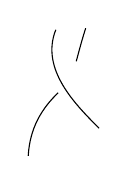
\begin{tikzpicture}
\draw (0.5,1.6) .. controls (0.3,1.1) and (0.75,0.65) .. (1.05,0.35);
\draw (0.15,0) .. controls (0.17,0.35) and (0.32,0.6) .. (0.53,0.8);
\draw (0.76,1.2) .. controls (0.8,1.35) and (0.84,1.5) .. (0.88,1.62);
\end{tikzpicture}
\end{adjustbox}

[Зачёркнуто: \Unclear{GELFAND-P001494}{spin-cancel}{неразборчиво}]

\underline{Спин?}

спин $\theta$

(в будущем)

\SourceFigure{GELFAND-P001494}{worldlines}{Две пары мировых линий с точками на концах: (1) две отдельные почти вертикальные линии; (2) вертикальная линия с разрывом внизу и изогнутая линия с двумя пересечениями. Цифры 1 и 2 обведены. Верхнее пересечение требует сверки со сканом.}

мировые линии

$\mathbb R_t^1\times\mathbb R^2$

[Справа: (в $\mathbb R^3$ и только в нём между ① и ② принцип. разница)]

\begin{equation*}
\begin{array}{c@{\qquad}c@{\qquad}c}
 & \text{①} & \text{②}\\
\text{Амплитуда} & 1 & e^{2\pi i\theta}
\end{array}
\end{equation*}
[Справа: (раньше $\theta$ — спин)]

Это прим. к квант. эфф. Холла.

При \Unclear{GELFAND-P001494}{last-line}{унесении?} вниз возникает сколько-то обходов.

\SourcePage{GELFAND-P001495}{unlabelled}
Что происх. с волновой ф-ей
\begin{equation*}
d>3\quad\Rightarrow\quad\theta=\frac{\text{integer}}{2}
\end{equation*}
\begin{equation*}
d=3\quad\Rightarrow\quad\theta\text{ — любое!}
\end{equation*}
\begin{equation*}
\Psi(x,y;T)=\int A_T(x,y\mid\tilde x,y)
\Psi(\tilde x,\tilde y\mid0)\,d\tilde x\,d\tilde y
\end{equation*}
\Unclear{GELFAND-P001495}{wave-arguments}{[В $A_T$ второй аргумент после черты — $y$ без отчётливой тильды.]}

[Под знаком интеграла зачёркнуто: \Unclear{GELFAND-P001495}{wave-cancel}{неразборчиво; возможно, дифференциалы}]

\begin{equation*}
A_T=\sum_{\substack{\text{по траект.}\\\text{частиц}}}
e^{L_1}e^{L_2}F(\text{траекторий})=
\end{equation*}
[Под $F(\text{траекторий})$ — скобка и повёрнутый знак равенства:]
\begin{equation*}
e^{2\pi i\theta\,(\text{индекс})}
\end{equation*}
(сколько раз захватились)

$\theta$ полуцелое кроме [вставлено: случая] $d=3$

\begin{equation*}
=\int \mathcal D\varphi\,\mathcal DA\quad
\exp\int_{d^3x}
|D\varphi|^2+\frac{1}{H}F_{\mu\nu}^2+
\epsilon_{\mu\nu\lambda}A_\mu F_{\nu\lambda}
\end{equation*}
\Unclear{GELFAND-P001495}{action-measure}{[Под внутренним интегралом: $d^3x$ / $d^3z$.]}
\Unclear{GELFAND-P001495}{action-denominator}{В знаменателе написан $H$-образный знак.}

[Под последним слагаемым:] \Unclear{GELFAND-P001495}{wess-caption}{Весс-Зуминовский член}

Эти же [вставлено: \Unclear{GELFAND-P001495}{inserted-word}{инт. / шт.}] можно использовать для высокотемпер. провод.

Виттен недавно использовал для опис. инвариантов узлов

(полиномы Джонса)

С. Шаташвили (ЛОМИ)

П. Вигман

\SourcePage{GELFAND-P001496}{unlabelled}
\underline{17/X-88г.}\quad \underline{Сем. Гельфанда.}

\underline{\underline{И.М. Гельфанд.}}\quad 1) \underline{Иерархия функционалов}

Локальные функционалы:
\begin{equation*}
S=\int_{t_0}^{t_1}H(q,p)\,dt
\end{equation*}

Ф-лы след. ступени: если вариация $\delta S$ локальна.

\quad (1-го рода)

[Справа, отделено двумя вертикальными штрихами: \underline{Пример:} $\lambda_1$]

Ф-лы 2-го рода: если $\delta S$ — 1-го рода.

[Зачёркнуто: Это] Это новый раздел типа гомологич. алгебры.

2) \underline{Квант. механика}: амплитуда
\begin{equation*}
e^{\frac{i}{\hbar}\int_{t_0}^{t_1}L(p,q)\,dt}
\end{equation*}

Прочитать дискуссию Эйнштейна и Бора о принципе неопределенности.

Надо написать
\begin{equation*}
\int e^{\frac{i}{\hbar}\int_{t_0}^{t_1}L(p,q)\,dt}\,Dp\,Dq
\end{equation*}

Метод стац. фазы.

\SourcePage{GELFAND-P001497}{unlabelled}
\underline{Задача}: вычислить приближенно
\begin{equation*}
\int_0^1(\sin 10^5x^3)\,dx
\end{equation*}

\underline{Увлекательная задача}: двойное изложение квантовой механики, на ней можно понять много математики

Читать надо: а) Ландау, Лифшиц «Кв. мех.»

\underline{\underline{Фейгин Б.}}\qquad \underline{Струны.}

\underline{Квант. механика}:

$M$ — мн-ие, $\forall$ отобр. окружности $S^1\to M$ ставится в соотв.
\begin{equation*}
e^{\frac{i}{\hbar}\int\frac{m\dot x^2}{2}\,dt}
=
e^{\frac{i}{\hbar}\int\mathcal L(x,\dot x)\,dt}
\tag{1}
\end{equation*}
и надо написать
\begin{equation*}
\int e^{\frac{i}{\hbar}\int\frac{m\dot x^2}{2}\,dt}\mathcal D x(t)
=
\int e^{\frac{i}{\hbar}\int\mathcal L(x,\dot x)\,dt}\mathcal D x(t)
\tag*{(1)'}
\end{equation*}

[Зачёркнуто: \Unclear{GELFAND-P001497}{middle-cancellation}{Част. / Чисто; замен.}\quad $\dot x^2\longrightarrow\mathcal L(x,\dot x)$.]

[Вписано и обведено, с указанием к следующей фразе: И даже]

\Unclear{GELFAND-P001497}{middle-conjunction}{а / и / знак наподобие \&} $\mathcal L$ надо взять более общим.

Пусть $M$ — симп. мн-ие

\quad $p,q$ — коорд., $H$ — ф-я на $M$

Напишем действие для траектории $p(t),q(t)$
\begin{equation*}
\int[H(p(t),q(t))\,dt-p\,dq]
\tag{2}
\end{equation*}
и
\begin{equation*}
\int e^{\frac{i}{\hbar}\int(H(p(t),q(t))-p\,dq)}\,Dp\,Dq
\tag{2'}
\end{equation*}
\Unclear{GELFAND-P001497}{phase-space-exponent}{[После $H(p(t),q(t))$ в (2′) множитель $dt$ не виден.]}

Подходы с пом. (1′) и (2′) связаны преобр. Лежандра

[Зачёркнуто: Теперь надо]

Более инвар. запись: $S^1\to M$
\begin{equation*}
\int e^{\frac{i}{\hbar}\left[\int_{S^1}H\,dt-\int_{\tikz[baseline=-0.4ex]{\draw (0,0) circle (0.09); \draw (-0.06,-0.04)--(0.01,0.08); \draw (-0.015,-0.08)--(0.055,0.065); \draw (0.04,-0.075)--(0.085,0.01);}}\omega\right]}
\tag{3}
\end{equation*}

[Справа:] ($\omega$ — симп. форма,

\tikz[baseline=-0.4ex]{\draw (0,0) circle (0.09); \draw (-0.06,-0.04)--(0.01,0.08); \draw (-0.015,-0.08)--(0.055,0.065); \draw (0.04,-0.075)--(0.085,0.01);} — [зачёркнуто: \Unclear{GELFAND-P001497}{disk-caption}{диск?}; вписано: пленка], натянутая на $S^1$

Обобщение (3) на случай струн в нек-ром частном случае —

— это \Unclear{GELFAND-P001497}{wess-word}{терм / термы} Весса — Зумино.

\SourcePage{GELFAND-P001498}{41}
\underline{И.М.Г. Преобр. Лежандра}: см. кн. Гельфанда — Фомина о вар. исчислении

\quad (добавление)

\quad (через волн. фронты)

\SourceFigure{GELFAND-P001498}{ray-diagram}{Слева: окружность около отмеченной точки $x_1$ и выходящая к $x_2$ кривая. На окружности есть разрывы и короткий крючкообразный штрих; направление возможной стрелки не установлено.}

В $\forall$ точке зад. «роза ветров»

Время дв-ния
\begin{equation*}
\int_{x_1}^{x_2}L(x,\dot x)\,dt
\end{equation*}
(не зав. от параметризации)

Берём волн. фронты.

Траект. — хар-ки.

[Разделительная черта.]

\underline{Ф.}\qquad $\mathcal E$ — риманово 2-мерн. мн-ие; $g_{ij}$ — метр. тензор на $\mathcal E$.

\underline{Своб. лагранжиан} (аналог $\dot x^2$)
\begin{equation*}
\mathcal L(X)=\int_{\mathcal E}\sqrt g\,g^{\alpha\beta}
\frac{\partial X^a}{\partial x^\alpha}
\frac{\partial X^b}{\partial x^\beta}G_{ab}\,dx^0\,dx^1
\tag{4}
\end{equation*}
\Unclear{GELFAND-P001498}{lagrangian-indices}{[Над $G$ зачёркнут верхний индекс; под ним виден $ab$.]}

$\{X^a(x^1,x^2)\}$ — вложение $\mathcal E$ в $\mathbb R^d$; $G^{ab}$ — метрика в $\mathbb R^d$

\Unclear{GELFAND-P001498}{measure-index}{[В $dx^0$ верхний знак густо обведён; ниже написаны $x^1,x^2$, а метрика обозначена $G^{ab}$.]}

Интеграл Фейнмана

[Слева перед (4′) зачёркнуто: \Unclear{GELFAND-P001498}{crossed-tag}{4?}]
\begin{equation*}
\int e^{\frac{i}{\hbar}\mathcal L(X)}\,\mathcal D X\,\mathcal D g
\tag{4'}
\end{equation*}

\underline{Вопрос И.М.Г.}: что такое преобр. Лежандра, связанное с поверхностями, а не с кривыми?

Это принципиальный и существ. вопрос

\underline{Теория Весса — Зумино.}

$\mathcal E$ с компл. структурой. Пишем в лок. координатах:

$z,\bar z$ — координаты
\begin{equation*}
\left.
\begin{aligned}
\frac{\partial}{\partial z}+A_0(z,\bar z)\\
\frac{\partial}{\partial\bar z}+A_1(z,\bar z)
\end{aligned}
\right\}\quad\text{связность}
\tag{5}
\end{equation*}

Выб. 3-мерн. плёнку, у к-рой $\mathcal E$ — край

Достраиваем [зачёркнуто: \Unclear{GELFAND-P001498}{extension-cancel}{до…?}] компон. (5) до плоских связностей
\begin{equation*}
\begin{aligned}
\left[\frac{\partial}{\partial\bar z}+B_0(z,\bar z),
\ \frac{\partial}{\partial z}+A_0(z,\bar z)\right]&=0\\
\left[\frac{\partial}{\partial z}+B_1(z,\bar z),
\ \frac{\partial}{\partial\bar z}+A_1(z,\bar z)\right]&=0
\end{aligned}
\tag{6}
\end{equation*}

(7) \underline{Условие}: \Unclear{GELFAND-P001498}{bottom-condition}{[Над строкой вставлено: Полученные плоские. В строке: Связн. прод.; далее зачёркнуто «до» и ниже ещё знак, возможно $\nabla_1$.]}
на плёнку как плоские связности $\nabla_1,\nabla_2$

\SourcePage{GELFAND-P001499}{unlabelled}
\underline{Лагранжиан:}
\begin{equation*}
\mathcal L(A_0,A_1)=
\int(A_0-B_1)(B_0-A_1)\,dz\wedge d\bar z+
WZ(\widetilde\nabla_1,\widetilde\nabla_2),
\tag{8}
\end{equation*}
[Под $WZ$: (Wess-Zumino)]

Выше исп. обозначения
\begin{equation*}
\nabla_1=\left\{\frac{\partial}{\partial z}+A_0,
\ \frac{\partial}{\partial\bar z}+B_0\right\},
\qquad
\nabla_2=\left\{\frac{\partial}{\partial z}+B_1,
\ \frac{\partial}{\partial\bar z}+A_1\right\};
\end{equation*}

$\widetilde\nabla_j$ — плоские продолжения $\nabla_j$ на плёнку
\begin{equation*}
WZ(\widetilde\nabla_1,\widetilde\nabla_2)=
\int_0^1\int_{\text{плёнке}}
\operatorname{tr}((\widetilde\nabla_1-\widetilde\nabla_2)
\cdot\Phi(t\widetilde\nabla_1+(1-t)\widetilde\nabla_2)\,dt
\tag{9}
\end{equation*}
\Unclear{GELFAND-P001499}{wz-integrand}{[После $\operatorname{tr}$ две открывающие круглые скобки; закрывающая внешняя скобка перед $dt$ не видна.]}

[От $\Phi$ штрих к подписи:]

кривизна

(форма [зачёркнуто: \Unclear{GELFAND-P001499}{curvature-caption}{неразборчивый зачёркнутый знак}] кривизны)

\underline{\underline{И.М. Гельфанд}}

\underline{Детерминант кубической матрицы.}

(по [зачёркнуто: \Unclear{GELFAND-P001499}{attribution-cancel}{Зелевин…?}] И.М.Г., Зелевинскому и Капранову)

\quad введение в будущий доклад

\begin{equation*}
a_{i,j,k},\quad i,j,k=1,2.
\end{equation*}
\begin{equation*}
\det\Vert\lambda a_{ij1}+\mu a_{ij2}\Vert
\end{equation*}
квадр. форма отн. $\lambda$ и $\mu$.

Берём её дискриминант по $\lambda,\mu$. Он наз. \underline{детерминантом} кубич. матрицы.

В $\det A$ есть действие $XAY$,

а в квадр. форме $X^*AX$.

Важно действие группы.

Вся теория групп возникла из понятия $\det$.

Из кубич. [зачёркнуто: \Unclear{GELFAND-P001499}{matrix-cancel}{неразборчиво}] матриц должны возникнуть новые объекты.

\underline{Представления $GL_n$ или $SL_n$.}

$N$ — \underline{унипот. подгруппа}; ${}_N\backslash G$ \Unclear{GELFAND-P001499}{quotient-corrections}{[После ${}_N\backslash G$ — две группы зачёркнутых знаков.]} — пр-во афф. флагов

(смотреть подробно $GL_2$); [зачёркнуто: \Unclear{GELFAND-P001499}{sl2-cancel}{неразборчиво; видны $G$, $A$, $G$-образные знаки}] $G=SL_2$ [зачёркнуто: \Unclear{GELFAND-P001499}{better-cancel}{неразборчиво}] лучше

На ${}_N\backslash G$ рассм. ф-ии (полиномы), однор. отн. левых сдвигов.

\SourcePage{GELFAND-P001500}{42}
\underline{Пример}: афф. плоскость и полиномы степ. $n$

Но: есть ещё дифф. формы; обозн. $B$ — пр-во форм $\omega$,

таких что $i_\lambda\omega=0$ \quad ($\lambda$ — элем. алг. Ли)

Теперь надо взять $B+dB$
\begin{equation*}
B=\bigoplus_{k,\mu} B_k(\mu)
\end{equation*}
[От $k$ штрих к подписи: пор. однор.; от $\mu$ штрих к подписи: степень формы.]
\begin{equation*}
C_0=C,\quad C_1=B_1(\bar\ell)+dB_0(\bar\ell),\ \ldots
\end{equation*}

Возник. кручение Уайтхеда: гипердет.

Повидимому, это позволяет заменить схемы Юнга.


\SourcePage{GELFAND-P001501}{unlabelled}
\underline{24.10.88 г.}\qquad \underline{\underline{Сем. Гельфанда}}

\underline{И.М.Г.}\quad \underline{Задачи по представлениям.}

Есть предст., [зачёркнуто: \Unclear{GELFAND-P001501}{cancel-first}{неразборчиво}] единичное; тавтологич. в $V$; в $S^2V$ (однор. мног. степ. 2).

Док. неприводимость $SL(2,R)$ в $S^3V$ (полиномы 3-й степени).

$\dim V=2$, в $V$ действ. тавтологич. предст.

Что для $SL(3,R)$? Это важная задача [зачёркнуто: \Unclear{GELFAND-P001501}{cancel-conjunction}{неразборчиво}] и её надо проделать.

\underline{Гипотеза:} тоже однородные полиномы [зачёркнут знак: \Unclear{GELFAND-P001501}{cancel-hypothesis}{неразборчиво}]?

Гельфанд, Наймарк

\underline{3 важные задачи}

1) $S_n$ (симм. группа)

2) $SL_n(R)$ --- конечномерные представления

3) $SO_n$ [зачёркнуто: \Unclear{GELFAND-P001501}{cancel-task-three-a}{неразборчиво}] столь же подробно, как [зачёркнуто: \Unclear{GELFAND-P001501}{cancel-task-three-b}{для \ldots}] в кн. Г.-М.-Ш. [ниже:] для $SO_3$.

\underline{Представления $SL(3,R)$.}

Ответ получен в кн. Гельф.-Наймарка «Унит. предст. классич. групп».

$N,B$ --- подгруппы в $G=SL(3,R)$.

\SourcePage{GELFAND-P001502}{46}
\begin{equation*}
\left\{\begin{pmatrix}1&0&0\\a_{21}&1&0\\a_{31}&a_{32}&1\end{pmatrix}\right\}=N
\tag{1}
\end{equation*}
\begin{equation*}
\left\{\begin{pmatrix}b_{11}&0&0\\b_{21}&b_{22}&0\\b_{31}&b_{32}&b_{33}\end{pmatrix}\right\}=B
\quad\text{(борелевская)}
\tag{2}
\end{equation*}
\begin{equation*}b_{11}b_{22}b_{33}=1.\end{equation*}
Рассм. классы смежности
\begin{equation*}
\underset{\displaystyle =\{Ng\mid g\in G\}}{N\backslash G}\quad\text{и}\quad B\backslash G
\tag{3}
\end{equation*}
(4) [Зачёркнуто: \Unclear{GELFAND-P001502}{cancel-assertion}{Теор.}] \underline{Утв.}
[Над $\forall$ вставлено: Почти.]
\begin{equation*}
\forall g\in G,\ \exists\text{ запись }g=nz,\quad\text{где }n\in N,\qquad
z=\begin{pmatrix}z_{11}&z_{12}&z_{13}\\0&z_{22}&z_{23}\\0&0&z_{33}\end{pmatrix}.
\end{equation*}
(обозн. $Z$ группу таких матриц)

(разлож. Гаусса)\qquad (верхне-треуг.)

Разлож. любой матр., обобщающее это, наз. \underline{разложением Брюа}.

[Зачёркнут начальный знак: \Unclear{GELFAND-P001502}{cancel-representatives}{неразборчиво}] Будем матр. $z$ использ. как представителей в $N\backslash G$.

Определим ф-и $f(z)$ [зачёркнуто: \Unclear{GELFAND-P001502}{cancel-functions}{неразборчиво}] на $N\backslash G$.

$Z\backslash G$ --- пр-во флагов. (ещё компактифицируем)
\Unclear{GELFAND-P001502}{flag-quotient}{В источнике $Z\backslash G$.}

\begin{equation*}
\begin{pmatrix}1&0\\\alpha&1\end{pmatrix}
\begin{pmatrix}a&b\\c&d\end{pmatrix}
=\begin{pmatrix}a&b\\\alpha a+c&\alpha b+d\end{pmatrix}
\end{equation*}
\begin{equation*}
\begin{pmatrix}z_{11}&z_{12}\\0&z_{12}^{-1}\end{pmatrix}
\end{equation*}
\Unclear{GELFAND-P001502}{inverse-index}{Нижний правый элемент записан как $z_{12}^{-1}$.}

Строим полином $f(z_{11},z_{12})$.

Для 3-го порядка нужно брать полиномы от 1-х 2-х строк, однородные по каждой. Надо рассм. их на простой компактификации.

\begin{equation*}
\lambda=\begin{pmatrix}\lambda_1&0&0\\0&\lambda_2&0\\0&0&\lambda_3\end{pmatrix}
\tag{5}
\end{equation*}
умн. [вставлено: слева] на $\lambda$ переводит класс в класс:
\begin{equation*}
g_1=ng_2\ \Rightarrow\ \lambda g_1=\lambda ng_2=
\underbrace{\lambda n\lambda^{-1}}_{n_1}\lambda g_2,\quad\text{ч.т.д.}
\end{equation*}
[Около $\Rightarrow$ зачёркнуто: \Unclear{GELFAND-P001502}{cancel-implication}{неразборчиво}.]

\SourcePage{GELFAND-P001503}{unlabelled}
\underline{Общее определение.}

$Z=N\backslash G$ --- основное аффинное пр-во.

Рассм. на $Z$ все аналит. ф-и. Это полиномы.

Рассм. ф-и, однор. относит. левых сдвигов:
\begin{equation*}
f(\lambda z)=\lambda_1^{k_1}\lambda_2^{k_2}\lambda_3^{k_3}f(z)
\tag{6}
\end{equation*}
\begin{equation*}(\lambda_1\lambda_2\lambda_3=1)\end{equation*}
\underline{Пр-во однор. полиномов конечномерно.}

$k_1,k_2,k_3$ --- старший вес предст.

\underline{Ф-лы для предст.:}
\begin{equation*}(T_gf)(z)=f(zg)\end{equation*}
[Зачёркнуто: \Unclear{GELFAND-P001503}{cancel-factor}{Можно профакторизовать по}.]

Предст. задаётся тройкой чисел $(k_1,k_2,k_3)$.

Задача: 1) когда предст. трив.?

2) когда предст. тавтологично?

3) когда оно [зачёркнуто: \Unclear{GELFAND-P001503}{cancel-symmetric}{в $S^2$}] эквив. предст. в $S^2V$?

Найти в этом пр-ве правильный базис.

Если старший вес $k$ правилен, то предст. реализуется в сечениях расслоения, т.е. в \Unclear{GELFAND-P001503}{cohomology-degree}{$H^0$ или $H^1$}.

Если же нет, то Ботт обнаружил, что предст. уходит в высшие когомологии пр-ва флагов.

\underline{Гельф., Зелевинский, Капранов.}

Важное наблюдение: на $Z$ надо рассматривать не только ф-и, но и дифф. формы!!!

Рассм. [вставлено: вект.] поле $\lambda$ и все формы [зачёркнут знак: \Unclear{GELFAND-P001503}{cancel-form-symbol}{$\lambda$?}] $\omega$, для к-рых $i_\lambda\omega=0$.

Здесь возникают супералгебры форм.

Нек-рые формы, к-рые важны:
\begin{equation*}
\Psi(z)\begin{vmatrix}z_1&z_2&z_3\\dz_1&dz_2&dz_3\\dz_1&dz_2&dz_3\end{vmatrix}
\end{equation*}
\begin{equation*}
\left|\begin{array}{ccc}
f_1(z)&f_2(z)&f_3(z)\\
z_1&z_2&z_3\\
dz_1&dz_2&dz_3\\
dz_1&dz_2&dz_3
\end{array}\right|
\end{equation*}
\Unclear{GELFAND-P001503}{rectangular-form}{Последняя запись имеет четыре строки и три столбца между вертикальными чертами.}

\SourcePage{GELFAND-P001504}{47}
Всё это связано с задачей о том, что такое $\det$.
\begin{equation*}
A=\begin{pmatrix}a_{11}&a_{12}&a_{13}\\a_{21}&a_{22}&a_{23}\\a_{31}&a_{32}&a_{33}\end{pmatrix}
\qquad \det A\text{ --- ?}
\end{equation*}
Знаменатель, возникающий при реш. лин. систем?

Что если $a_{ij}$ некоммутируют?

Другой подход.

Векторы можно преобразовывать действием группы $GL_n$.

Есть 2 [зачёркнуто: \Unclear{GELFAND-P001504}{cancel-orbits}{неразборчиво}] орбиты: $0$ и $V\setminus\{0\}$.

Пусть $X,Y$ --- невыр. матрицы. Можно заменить $A$ на $XAY$. Тогда все невыр. матрицы эквивалентны.

$\det$ --- ф-я $f(A)$, обращ. в $0$ на особых матр.

Или:
\begin{equation*}\sum a_{ik}\xi_i\eta_k\end{equation*}
[Между $\xi_i$ и $\eta_k$ зачёркнут знак: \Unclear{GELFAND-P001504}{cancel-bilinear}{$\eta$?}.]

на $\xi$ действует $X$, а на $\eta$ --- $Y$.

$\det$ --- [вставлено: однор.] ф-я от коэфф. $(a_{ij})$ наименьшей степ., равная $0$ на всех особых поверхностях.

(Всё это на проективных пр-вах).

Рассм. кубич. матрицу $a_{ijk}$ и [зачёркнуто: \Unclear{GELFAND-P001504}{cancel-cone}{ф-му?}] конус
\begin{equation*}\sum a_{ijk}\xi_i\eta_j\zeta_k=0\tag{7}\end{equation*}
в проектив. пр-ве.

Куб. $\det$ --- однор. ф-я наименьшей степ. от $a_{ijk}$, равная $0$ на особых поверхностях.

2-мерн. случай: сделал Кэли, но с ошибкой.

$i,j,k=1,2$.

\SourceFigure{GELFAND-P001504}{cube}{Куб в косоугольной проекции. Передняя грань: снизу слева $000$, снизу справа $001$, сверху справа $101$, сверху слева $100$. На сдвинутой вверх и вправо задней грани соответственно $010$, $011$, $111$, $110$; часть скрытых рёбер пунктирная. На верхнем переднем ребре короткие дополнительные штрихи, направление возможных стрелок не установлено.}

$\operatorname{deg}=4$.

Элем. 3-х типов:

1) квадраты (6 штук):
\begin{equation*}\sum\text{произв. по квадратам}\end{equation*}
2) \SourceFigure{GELFAND-P001504}{antiquadrats}{Два небольших наброска: слева густо перечёркнутая угловатая фигура, справа две пересекающиеся диагонали, одна с разрывом около пересечения. Связь отдельных штрихов и зачёркивания требует сверки с оригиналом.}
антиквадраты (впис. тетраэдр)

(2 штуки)

\SourcePage{GELFAND-P001505}{unlabelled}
3) $\sum$ [зачёркнуто: по ди] $a^2b^2$ [под суммой: по диагоналям] (4 штуки)

\begin{equation*}
\begin{aligned}
\operatorname{Det}(a_{ijk})={}&
\left(
\begin{vmatrix}a_{111}&a_{212}\\a_{121}&a_{222}\end{vmatrix}
+\begin{vmatrix}a_{211}&a_{112}\\a_{221}&a_{122}\end{vmatrix}
\right)^2\\
&-4\begin{vmatrix}a_{111}&a_{112}\\a_{121}&a_{122}\end{vmatrix}
\cdot\begin{vmatrix}a_{211}&a_{212}\\a_{221}&a_{222}\end{vmatrix}
\end{aligned}
\tag{8}
\end{equation*}
[Знак «−» повторён в конце первой и начале второй строки.]

Рассм. 2 матрицы $A_1$ при $k=1$, $A_2$ при $k=2$.
\Unclear{GELFAND-P001505}{slice-index}{В обозначении срезов написано $k=1$, $k=2$.}

$\det|\xi_1A_1+\xi_2A_2|$ --- квадр. форма от $\xi_1,\xi_2$.
\begin{equation*}
\text{Дискр.}\,[\det(\xi_1A_1+\xi_2A_2)]=(8).
\tag{9}
\end{equation*}
Из (9) не очевидна симметричность по всем индексам.

$(a_{ijk})$ --- произв. предст. $SL_n\times SL_n\times SL_n$

(по 3-м индексам)

(тензорное произв. трёх тавтологич. представлений)

\underline{Гипотеза:} $\det$ --- кручение Уайтхеда комплекса Кэли--Кошуля (см. стр. 42).

\underline{Другой подход}

Рассм. вложение
\begin{equation*}
X=P^{m_1-1}\times P^{m_2-1}\times P^{m_3-1}\subset P^{m_1m_2m_3-1}=P
\end{equation*}
по Сегре (зад. пучком $O(1,1,1)$) --- полилинейными формами.

[Слева над следующей строкой, с линией к $\check X$:] Двойств. [зачёркнуто: \Unclear{GELFAND-P001505}{cancel-dual}{неразборчиво}] \Unclear{GELFAND-P001505}{dual-abbreviation}{мн-же?}

Тогда $\check X\subset\check P$.

$\check X$ --- гиперповерхность. $\operatorname{deg}$ --- ? Уравнение --- ?

$\check P$ --- пр-во гиперплоскостей в $P$.

$\check X$ --- мн-во гиперпл., касающихся $X$ в какой-нибудь точке.

[Выделено скобкой:] касание:
\begin{equation*}
\pi\text{ касается }X\ \Leftrightarrow\ T_x\pi\supset T_xX
\end{equation*}
Надо читать Клейна

а) Ист. разв. матем.

б) Высш. геом.

в) Элем. мат. с точки зр. высшей.

Изом. моделей Пуанкаре и Клейна для $H^2$?

[Над «Пуанкаре»: (окр. с сохр. углов). Над «Клейна»: \Unclear{GELFAND-P001505}{klein-model-note}{(окр. с \ldots\ уг.)}.]

\SourcePage{GELFAND-P001506}{48}
\begin{equation*}
N_d(2)=(-1)^d\sum_{i=0}^d(i+1)(-1)^i2^{d-i}\binom di i!
\tag{10}
\end{equation*}
(степень $\det$ в $d$-мерном пр-ве)

[Ниже вставлено:] матриц $\underbrace{2\times2\times\ldots\times2}_{d\text{ раз}}$.

Правильная ф-ла:
\begin{equation*}
N_d(2)=(d+3)d!e_d(-2)+(d+1)(-2)^d\in Z,
\tag{11}
\end{equation*}
где
\begin{equation*}e_d(z)=\sum_{k=0}^{d-1}\frac{z^k}{k!}.\end{equation*}
\begin{equation*}
N_d(2)\sim\frac{(d+3)d!}{e^2}\quad\text{при больших }d
\end{equation*}
\begin{equation*}
\begin{array}{c|cl}
d&N_d(2)&\\
2&2&\\
3&4&\\
4&24&\text{(Шлефли)}\\
5&128&
\end{array}
\end{equation*}

\underline{\underline{А.С. Шварц.}}

Некоммут. аналог кручения Рэя--Зингера.

Идея постр. топ. инвариантов в КТП

Действие
\begin{equation*}S(A)=\int_{M^3}A\wedge dA\tag{1}\end{equation*}
[В номере после $1$ зачёркнута цифра: \Unclear{GELFAND-P001506}{cancel-action-number}{2?}. Справа зачёркнуто: \Unclear{GELFAND-P001506}{cancel-gauge}{А --- кали\ldots}.]

даёт кручение Рэя--Зингера.

Есть обобщение, когда $A$ --- форма со знач. в алг. Ли $\mathfrak g$

(калибр. поле или связность в главном расслоении (тривиальном))

$M^3\times G$

$G$ --- компактная группа Ли
\begin{equation*}
S(A)=\operatorname{Tr}\int_{M^3}A\wedge dA
+\frac23\operatorname{Tr}\int_{M^3}A\wedge A\wedge A
\tag{2}
\end{equation*}
[Под вторым слагаемым:] $\operatorname{Tr}[A,A]\wedge A$

надо рассм. стат. сумму
\begin{equation*}Z=\int e^{-S(A)}\tag{3}\end{equation*}
\begin{equation*}
\delta S=0\quad\text{(ур-е дв-ния)}\quad\Leftrightarrow\quad F=0
\tag{4}
\end{equation*}
[После $\delta S=0$ зачёркнуто: \Unclear{GELFAND-P001506}{cancel-motion}{ур?}. Под $F$:] кривизна связности.

\SourcePage{GELFAND-P001507}{unlabelled}
Можно записать
\begin{equation*}
S(A)=\int_{N^4}F\wedge F,\qquad\partial N=M
\tag{5}
\end{equation*}
(продолжаем связность $A$ на $N^4$ и берём кривизну $F$)

Здесь возникают \Unclear{GELFAND-P001507}{topological-word}{топ.?}.

Зацепления $\rightsquigarrow$ окр. узла, [зачёркнуто: \Unclear{GELFAND-P001507}{cancel-gluing}{её?}] склеиваем с дублем --- получ. $M^3$.

Рассм. ещё

[Зачёркнуто: $\operatorname{Tr}$]
\begin{equation*}P\exp\oint_\Gamma A\,dx\quad\text{(монодромия)}\end{equation*}
и модифицируем

[Слева от номера (6) ещё одна открывающая скобка.]
\begin{equation*}S(A)=\int e^{-S(A)}\operatorname{Tr}P\exp\oint_\Gamma A\,dx\tag{6}\end{equation*}
\Unclear{GELFAND-P001507}{modified-action}{Слева в (6) написано $S(A)$.}

\SourcePage{GELFAND-P001508}{53}
\underline{31/X-88.}\qquad\underline{Сем. Гельфанда.}

\underline{В.Е. Захаров.}\quad Ур-я гидродинамики в форме Клебша.

Пусть $S$ --- матрица из полупр. алг. Ли. Рассм. ур-е
\begin{equation*}
\frac{\partial S}{\partial t}=\left[S,\frac{\partial H}{\partial S}\right]
=S_{\alpha\gamma}\frac{\partial H}{\partial S_{\gamma\beta}}
-\frac{\partial H}{\partial S_{\alpha\gamma}}S_{\gamma\beta}
\tag{1}
\end{equation*}
[После второго знака равенства зачёркнуто: \Unclear{GELFAND-P001508}{cancel-commutator}{$H$?}.]

\begin{equation*}\operatorname{Sp}S^n=I_n\quad\text{--- интегр. дв-ния}\tag{2}\end{equation*}
\begin{equation*}S=[p,q],\qquad H=H(S)=H(p,q]\tag{3}\end{equation*}
\Unclear{GELFAND-P001508}{hamilton-bracket}{Конечная скобка в $H(p,q]$: квадратная или угловатая круглая.}

($p,q$ --- буквы)
\begin{equation*}
\left\{\begin{aligned}
\dot p&=\left[p,\frac{\partial H}{\partial S}\right]=-\frac{\partial H}{\partial q},\\
\dot q&=\left[q,\frac{\partial H}{\partial S}\right]=\frac{\partial H}{\partial p}.
\end{aligned}\right.\tag{4}
\end{equation*}
\begin{equation*}\operatorname{Sp}(p^{n_1}q^{n_2}p^{n_3}\ldots)=\operatorname{const}\quad\text{--- интегралы.}\tag{5}\end{equation*}
\underline{Переменные Клебша}

$\varphi(x,y)$
\begin{equation*}A=-\varphi_y\frac{\partial}{\partial x}+\varphi_x\frac{\partial}{\partial y}\tag{6}\end{equation*}
Пусть есть 2 таких $A_1,A_2$.

Тогда
\begin{equation*}[A_1,A_2]=-\varphi_{3y}\frac{\partial}{\partial x}+\varphi_{3x}\frac{\partial}{\partial y}\tag{7}\end{equation*}
\begin{equation*}\varphi_{3x}=\varphi_{1x}\varphi_{2y}-\varphi_{1y}\varphi_{2x}=\{\varphi_1,\varphi_2\}\end{equation*}
\Unclear{GELFAND-P001508}{phi-three-index}{Слева в определении скобки написано $\varphi_{3x}$.}

\underline{Ур-я гидродинамики в форме Клебша}
\begin{equation*}\frac{\partial\Omega}{\partial t}+\{\Psi,\Omega\}=0\tag{8}\end{equation*}
[Справа зачёркнут знак: \Unclear{GELFAND-P001508}{cancel-margin}{неразборчиво}.]

$v_x,v_y,\quad\operatorname{div}v=0$
\begin{equation*}v_x=-\Psi_y,\quad v_y=\Psi_x\quad(\Psi\text{ --- ф-я тока})\tag{9}\end{equation*}
\begin{equation*}\Omega=\Delta\Psi\tag{10?}\end{equation*}
\Unclear{GELFAND-P001508}{overwritten-ten}{Номер переправлен; чтение (10) предположительно, предшествующие штрихи неразборчивы.}

\begin{equation*}\dot H=\frac12\int v^2\,d\vec r=-\frac{\delta H}{\delta\Omega}\tag{11}\end{equation*}
\Unclear{GELFAND-P001508}{energy-chain}{Над $H$ точка; в строке сохранено равенство интеграла и $-\delta H/\delta\Omega$.}

(гамильт. запись 2-мерн. гидродин.)

С 1844 г. известно [ниже вставлено: (Клебш)] ([над скобкой:] \Unclear{GELFAND-P001508}{lamb-insertion}{ур.} Лэма и др.)

Пусть $\Omega=\{\lambda,\mu\}$. Получится аналогично (4):

[Под $\{\lambda,\mu\}$:] (скобка Пуасс.)

\SourcePage{GELFAND-P001509}{unlabelled}
Получится:
\begin{equation*}
\left\{\begin{aligned}
\frac{\partial\lambda}{\partial t}+\{\Psi,\lambda\}&=0\\
\frac{\partial\mu}{\partial t}+\{\Psi,\mu\}&=0
\end{aligned}\right.
\quad\left|\quad
\left\{\begin{aligned}
\frac{\partial\lambda}{\partial t}&=-\frac{\delta H}{\delta\mu}\\
\frac{\partial\mu}{\partial t}&=\frac{\delta H}{\delta\lambda}
\end{aligned}\right.\right.\tag{12}
\end{equation*}
Интегралы дв-ния?

У нас
\begin{equation*}\Psi=-\frac{\delta H}{\delta\Omega}\tag{13}\end{equation*}
и
\begin{equation*}\frac{\partial\Omega}{\partial t}+\{\Psi,\Omega\}=0\tag{14}\end{equation*}
(15) \underline{Лемма 1.} Если
\begin{equation*}\frac{\partial\lambda_i}{\partial t}+\{\Psi,\lambda_i\}=0,\qquad i=1,2,\tag{16}\end{equation*}
то $\{\lambda_1,\lambda_2\}$ удовл. тому же ур-ю
\begin{equation*}\frac{\partial}{\partial t}\{\lambda_1,\lambda_2\}+\{\Psi,\{\lambda_1,\lambda_2\}\}=0.\tag{17}\end{equation*}
\underline{Лемма 2.}

Если $\lambda_i$, $i=1,\ldots,N$ удовл. (16), то
\begin{equation*}\int F(\lambda_1,\ldots,\lambda_N)\,d\vec r=\operatorname{const}\quad\text{--- интегралы дв-ния}\tag{18}\end{equation*}
Итак, сохраняются
\begin{equation*}\int F(\lambda,\mu,\Omega,\{\lambda,\Omega\},\{\mu,\Omega\},\ldots)\,d\vec r\tag{19}\end{equation*}
Алгебра Ли ф-лов (19) (отн. «скобки Пуасс.») сод. подалгебру (!)
\begin{equation*}J_0=\left\{\int F(\lambda,\mu)\,d\vec r\right\}\tag{20}\end{equation*}
\begin{equation*}
\begin{aligned}
[J_0^1,J_0^2]&=\int(F^1_\lambda F^2_\mu-F^1_\mu F^2_\mu)\,d\vec r\\
&=\int\langle F_1,F_2\rangle\,d\vec r
\end{aligned}\tag{21}
\end{equation*}
\Unclear{GELFAND-P001509}{poisson-last-index}{Последний множитель в скобках записан $F^2_\mu$, не $F^2_\lambda$.}

[Под $\langle F_1,F_2\rangle$:] обычная скобка Пуасс. на фаз. пр-ве

Рассм. алгебру
\begin{equation*}J_1=\left\{\int F(\lambda,\mu,\Omega)\,d\vec r\right\}\tag{22}\end{equation*}
Это будет алгебра токов над алг. (20).

\SourcePage{GELFAND-P001510}{54}
Рассм.
\begin{equation*}
J_1^n=\int F_1(\lambda,\mu)\Omega^n\,d\vec r,\qquad
J_2^m=\int F_2(\lambda,\mu)\Omega^m\,d\vec r
\tag{23}
\end{equation*}
\begin{equation*}
[J_1^n,J_2^m]=\frac{(n-1)(m-1)}{n+m-1}\int\langle F_1^n,F_2^m\rangle\Omega^{n+m}\,d\vec r
\tag{24}
\end{equation*}
\Unclear{GELFAND-P001510}{current-bracket}{Сохранены верхние индексы $n,m$ у $F_1,F_2$ и степень $\Omega^{n+m}$.}

(получ. алг. Вирасоро с 0-м центр. зарядом)

Есть 2-парам. набор интегралов. Интегрируемости в общ. случае нет ($H$ произвольно!!) Какая неполнота?

Попробуем применить теор. Лиувилля.

Будем делать замены перем.
\begin{equation*}
x'=x'(x,y),\quad y'=y'(x,y),\qquad\frac{\partial(x',y')}{\partial(x,y)}=1
\tag{25}
\end{equation*}
сохр. площадь. Все интегр. (23) от этого не меняются.

Фиксируем $\lambda$; какие замены сохр. $\lambda$

Надо скользить по линиям уровня $\lambda$; $\varphi=f(\lambda)$.

Введём
\begin{equation*}a_k=\frac1{\sqrt2}(\lambda_k+i\mu_k)\end{equation*}
и рассм. гамильтониан
\begin{equation*}H=\int W_{kk_1,k_2k_3}\bar a_k\bar a_{k_1}a_{k_2}a_{k_3}\tag{26}\end{equation*}
При его спец. форме (точно сейчас не выписывается)
\begin{equation*}
W'(k,k_1,k_2,k_3)=\{k_1,k_2\}\{k_2,k_3\}f(k_1-k_3)+\ldots
\tag{27}
\end{equation*}
\Unclear{GELFAND-P001510}{w-first-argument}{После первого $k$ густой переправленный знак: запятая либо нижний индекс с запятой.}

$(28)_1$ [Зачёркнуто: Для] При $f=\dfrac1{k^2}$ не хватает интегралов.

$(28)_2$ При $f=\dfrac{\vec\alpha\,\vec k}{\vec\beta\,\vec k}$ получ. $\infty$-мерн. волчок и интегрируется.

Захаров хочет провести числ. эксперимент о появлении хаоса.

[Вставлено слева:] В 3-мерном случае
\begin{equation*}\vec\Omega=[\vec A,\operatorname{rot}\vec B]-[\vec B,\operatorname{rot}\vec A]\end{equation*}
Это вектор и не появляется интегралов в дост. количестве.

В начале след. семинара Захаров расскажет о турбулентности.


\SourcePage{GELFAND-P001511}{unlabelled}
\underline{И. М. Гельфанд.}

[Под именем зачёркнуто и заштриховано:
\Unclear{GELFAND-P001511}{heading-cancelled}{неразборчиво}.]

\underline{Двойственная кривая}

\begin{equation*}
y=kx+b
\end{equation*}
\begin{center}
\begin{adjustbox}{max width=\linewidth}
\begin{tikzpicture}[x=1cm,y=1cm]
\draw[->] (1.1,0) -- (-1.1,0);
\draw (0,-0.5) -- (0,0.9);
\node at (1.12,-0.22) {$x$};
\node at (-0.22,1.05) {$y$};
\draw[->] (5.4,0) -- (3.2,0);
\draw (4.2,-0.45) -- (4.35,0.9);
\node at (5.65,-0.24) {$k$};
\node at (4.1,1.12) {$b$};
\end{tikzpicture}
\end{adjustbox}
\end{center}

это неудобно, т.к. $k$ и $b$ имеют разную размерность.

\begin{equation*}
\frac{x}{a}+\frac{y}{b}=1
\qquad \text{тоже не вполне удовлетворительно.}
\end{equation*}
Лучше:
\begin{equation*}
\xi x+\eta y=1
\end{equation*}
\begin{center}
\begin{adjustbox}{max width=\linewidth}
\begin{tikzpicture}[x=1cm,y=1cm]
\draw[->] (0.55,0) -- (-0.7,0);
\draw (0,-0.48) -- (0,0.57);
\node at (0.9,-0.2) {$x$};
\node at (-0.26,0.77) {$y$};
\draw[->] (5.55,0) -- (3.8,0);
\draw (4.65,-0.45) -- (4.78,0.6);
\node at (5.65,-0.3) {$\xi$};
\node at (4.52,0.82) {$\eta$};
\end{tikzpicture}
\end{adjustbox}
\end{center}

Прямая — точка на плоскости $\xi,\eta$

Аналогично:
\begin{equation*}
\xi_1x_1+\ldots+\xi_nx_n=1
\qquad\text{— гиперплоскость.}
\end{equation*}

Тогда

двойств. кривая образована всеми касательными на плоск. $(\xi,\eta)$

\underline{Пример 1.} $y=x^3$
\begin{gather*}
y-y_0=3x_0^2(x-x_0)\\
k=3x_0^2,\quad b=-2x_0^3
\end{gather*}
\begin{center}
\begin{adjustbox}{max width=\linewidth}
\begin{tikzpicture}[x=1cm,y=1cm]
\draw[->] (1,0) -- (-1.2,0);
\draw (0,-0.82) -- (0,1.08);
\draw (-0.98,-0.82) .. controls (-0.78,-0.13) and (-0.4,-0.13) .. (0,0)
.. controls (0.56,0.17) and (0.52,0.34) .. (0.72,1.08);
\draw[->] (5.25,-0.1) -- (2.9,-0.1);
\draw (4.25,-0.85) -- (4.25,0.92);
\draw (3.48,0.77) .. controls (4.04,0.71) and (4.14,0.39) .. (4.25,-0.1)
.. controls (4.34,0.53) and (4.55,0.83) .. (5.17,0.99);
\node at (4.82,-1.16) {двойств. кривая};
\end{tikzpicture}
\end{adjustbox}
\end{center}

Отсюда можно понять преобр. Лежандра.

\underline{Пример 2.}
\begin{equation*}
|x|^p+|y|^p=1
\end{equation*}
Лучше всего взять
\begin{equation*}
\xi x+\eta y=1\qquad\text{и узнать, когда касается.}
\end{equation*}
Получается
\begin{equation*}
|\xi|^{q}+|\eta|^q=1,\qquad\text{где}\quad\frac{1}{p}+\frac{1}{q}=1
\end{equation*}
[Первый показатель обведён и исправлен:
\Unclear{GELFAND-P001511}{exponent-overwrite}{$q$; прежний знак неразборчив}.]

(двойств. банахово пр-во)

\underline{Задача} (для любителей геометрии бан. пр-в)

В кубе большой размерности есть сечение, сколь угодно близкое к окружности.

\underline{Компл. точка зрения.}

Двойств. мн-ие — кас. плоскости

\SourcePage{GELFAND-P001512}{55}
В $\mathbb{C}^3$:
\begin{equation*}
\underline{\text{прямая}}\quad\longleftrightarrow\quad\underline{\text{прямая}}
\end{equation*}

Размерность двойств. мн-ия — важная задача.

\underline{Задача} Рассм. пр-во
\begin{equation*}
\mathbb{P}^{(m_1-1)}\times\mathbb{P}^{(m_2-1)}\times\ldots\times\mathbb{P}^{(m_k-1)}
\subset\mathbb{P}^{m_1m_2\ldots m_k-1}
\end{equation*}

[Зачёркнуто: Задача.] Задача о гипердетерминантах эквив. след. задаче:

когда двойств. поверхность имеет $\operatorname{codim}=1$?

Левая часть ур-я, задающего двойств. пов. — гипердетерминант.

Степень — ?

Гельфанд и соавторы могут это вычислить. Ответ таков: для
\begin{equation*}
\mathbb{P}^{\ell_1}\times\mathbb{P}^{\ell_2}\times\ldots\times\mathbb{P}^{\ell_d}
\subset\mathbb{P}^{(\ell_1+1)(\ell_2+1)\ldots(\ell_d+1)-1}
\end{equation*}
степень многочл., зад. [зачёркнуто:
\Unclear{GELFAND-P001512}{degree-cancelled}{ф?}] её, будет
\begin{equation}
N(\ell_1,\ell_2,\ldots,\ell_d)
=\sum_{\substack{0\le k_1\le\ell_1\\\ldots\\0\le k_d\le\ell_d}}
(-1)^{\sum(\ell_i-k_i)
\Bigl[(s+1)\prod_{i=1}^{d}\binom{s}{k_i}\binom{s+1+\ell_i-k_i}{\ell_i-k_i}
-s\prod_{i=1}^{d}\binom{s-1}{k_i}\binom{s+\ell_i-k_i}{\ell_i-k_i}}
\tag{1}
\end{equation}
\Unclear{GELFAND-P001512}{degree-formula-layout}{[Верхнее положение всего продолжения после $(-1)$ воспроизводит расположение записи. Неясно, относится ли к показателю только $\sum(\ell_i-k_i)$ или также следующее выражение. Закрывающая квадратная скобка не видна.]}

\begin{equation*}
s=k_1+\ldots+k_d
\end{equation*}

\underline{Лещинер Д.}

Производ. ф-я для этого числа
\begin{equation}
\begin{aligned}
\sum N(\ell_1,\ldots,\ell_d,\ldots)\,
\text{\Unclear{GELFAND-P001512}{generating-first-variable}{$x_1$ или $z_1$}}^{\ell_1}
x_2^{\ell_2}\ldots x_d^{\ell_d}x_{d+1}^{0}\ldots
=\left(\sum_{k=0}^{\infty}(1-k)e_k\right)^{-2}
\end{aligned}
\tag{2}
\end{equation}
[Между $x_2^{\ell_2}$ и многоточием зачёркнуто:
\Unclear{GELFAND-P001512}{generating-cancelled}{$\ell$?}.]

(после $\ell_d$ приписываем нулей
\Unclear{GELFAND-P001512}{generating-parenthesis-ending}{неразборчиво; возможно, «сколько.»})

\begin{equation*}
e_0=1
\end{equation*}

$e_k$ — элем. симметрич. ф-и:
\begin{align*}
e_1&=\sum_i x_i,\\
e_2&=\sum_{i<j}x_ix_j\\
e_3&=\sum_{i<j<k}x_ix_jx_k\\
&\ldots
\end{align*}

\underline{Капранов М.} Другая ф-ла:
\begin{equation*}
\lambda=(\ell_1\ge\ell_2\ge\ldots)
\end{equation*}
\begin{equation*}
N(\lambda)=\sum_{\mu}
\frac{(m_1+1)!\,\prod_{i\ge1}(i-1)^{m_i-m_{i+1}}}
{(m_1-m_2)!\,(m_2-m_3)!\ldots}\cdot M(\mu',\lambda),
\end{equation*}
\begin{equation*}
\mu=(m_1\ge m_2\ge\ldots)
\end{equation*}

\SourcePage{GELFAND-P001513}{unlabelled}
где $\mu'$ — двойств. разбиение

\SourceFigure{GELFAND-P001513}{upper-partition-diagram}{Ступенчатая диаграмма с общей левой стороной: три горизонтальные полосы, верхняя самая длинная, средняя короче, нижняя короткая. В полосах сверху вниз стоят $m_1$, $m_2$, $m_3$. Под диаграммой слева направо повёрнуты подписи $m'_1$, $m'_2$, $m'_3$, $m'_4$; первая подпись переправлена. Над верхней полосой зачёркнута ещё одна подпись, похожая на $m_1$; её исходное начертание неразборчиво.}

$M(\mu',\lambda)$ — число матриц из $0$ и $1$, у к-рых суммы по строкам и по столбцам

\begin{center}
\begin{adjustbox}{max width=\linewidth}
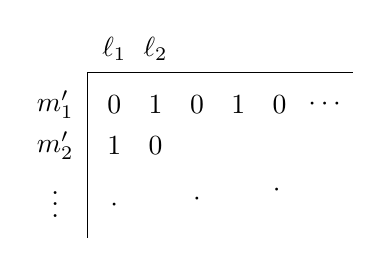
\begin{tikzpicture}[x=0.75cm,y=0.75cm]
\draw (0,0)--(0,2.8)--(4.5,2.8);
\node at (0.45,3.2) {$\ell_1$};
\node at (1.15,3.2) {$\ell_2$};
\node at (-0.55,2.25) {$m'_1$};
\node at (-0.55,1.55) {$m'_2$};
\node at (-0.55,0.7) {$\vdots$};
\node at (0.45,2.25) {$0$};
\node at (1.15,2.25) {$1$};
\node at (1.85,2.25) {$0$};
\node at (2.55,2.25) {$1$};
\node at (3.25,2.25) {$0$};
\node at (4.05,2.25) {$\cdots$};
\node at (0.45,1.55) {$1$};
\node at (1.15,1.55) {$0$};
\node at (0.45,0.55) {$\cdot$};
\node at (1.85,0.65) {$\cdot$};
\node at (3.2,0.8) {$\cdot$};
\end{tikzpicture}
\end{adjustbox}
\end{center}

\begin{equation*}
M(\mu',\lambda)>0\quad\Rightarrow\quad\lambda\ge\mu
\quad\text{относит. естеств. порядка.}
\end{equation*}
и, более того, тогда
\begin{equation*}
\forall i:\quad \ell_i\le\sum_{j\ne i}\ell_j
\end{equation*}

\underline{Зелевинский}

Погран. случай:
\begin{equation*}
\ell_1=\ell_2+\ldots+\ell_d
\end{equation*}
Тогда
\begin{equation*}
N=\frac{(\ell_1+1)!}{\ell_2!\ell_3!\ldots\ell_d!}
\end{equation*}
Видимо, здесь и надо считать $\det$

(1-й нетрив. случай: [зачёркнуто: \Unclear{GELFAND-P001513}{bottom-cancelled-sign}{неразборчивый знак}] $2\times3\times4$)

\SourcePage{GELFAND-P001514}{unlabelled}
\underline{13/$\overline{\mathrm{II}}$-88.}

\underline{\underline{Зелевинский}}. \underline{О} \underline{многомерных} \underline{детерминантах.}

\begin{equation*}
A=(a_{i_1\ldots i_d})_{0\le i_k\le\ell_k}
\quad\text{— многомерная матрица}
\end{equation*}
\begin{equation*}
\dim V_k=\ell_k+1;\qquad x_i^{(1)}\in V_1,\ldots,x_i^{(d)}\in V_d.
\end{equation*}
\begin{equation*}
A\in(V_1\otimes\ldots\otimes V_d)^*
\end{equation*}
\begin{equation*}
x\ \Unclear{GELFAND-P001514}{tensor-equality}{=\,/\,\ne}\ x^{(1)}\otimes\ldots\otimes x^{(d)}
\end{equation*}
\begin{equation*}
A(x)=\sum_{i_1,\ldots,i_d}a_{i_1\ldots i_d}\Unclear{GELFAND-P001514}{coefficient-stroke}{\text{короткий штрих: }-\text{ или соединение}}x_{i_1}^{(1)}\ldots x_{i_d}^{(d)}
\end{equation*}
\begin{equation*}
\operatorname{Det} A=0\quad\Longleftrightarrow\quad A\text{ — вырожденная}
\end{equation*}
\begin{equation*}
A\text{ — вырожд.}\quad\overset{\mathrm{def}}{\Longleftrightarrow}\quad
\exists x^{(1)},\ldots,x^{(d)}\ne0
\end{equation*}
\begin{equation*}
\ell_1\ge\ell_2,\ell_3,\ldots,\ell_d
\end{equation*}
\begin{equation*}
A(x^{(1)},\ldots,x^{(i-1)},\cdot,x^{(i+1)},\ldots,x^{(d)})\equiv0
\quad\text{для всех }i
\end{equation*}
\begin{equation*}
\begin{aligned}
\det\text{ имеет смысл}\quad &\overset{\mathrm{def}}{\Longleftrightarrow}\quad
\operatorname{codim}\{\text{вырожд. матриц}\}=1\\
&\qquad\Updownarrow\\
&\qquad\ell_1\le\ell_2+\ell_3+\ldots+\ell_d
\end{aligned}
\end{equation*}
\begin{equation*}
(\ell_1+1)\times(\ell_1+1)\quad\Rightarrow\quad\operatorname{deg}=\ell_1+1
\end{equation*}

(1) \underline{Утв.} Пусть $\ell_1=\ell_2+\ldots+\ell_d$

Тогда $\operatorname{Det}$ имеет степень
\begin{equation*}
\frac{(\ell_1+1)!}{\ell_2!\ell_3!\ldots\ell_d!}
\end{equation*}
Пусть Степень $\operatorname{Det}$ для $(\ell_1+1)\times\ldots\times(\ell_d+1)$
есть $N(\ell_1,\ldots,\ell_d)$

и $N(\ell_1,\ldots,\ell_d)=0$, если $\operatorname{Det}$ не имеет смысла

\SourcePage{GELFAND-P001515}{69}
(2) \underline{Утв.}
\begin{equation*}
\begin{aligned}
\sum_{\ell_1,\ldots,\ell_d\ge0}N(\ell_1,\ldots,\ell_d)x_1^{\ell_1}\ldots x_d^{\ell_d}
&=\\
&=\left[1-\sum_{i\ge2}(i-1)e_i(x_1,\ldots,x_d)\right]^{-2},
\end{aligned}
\end{equation*}
где $e_i$ — элем. симм. многочлен
\begin{equation*}
e_i(x_1,\ldots,x_d)=\sum_{k_1<\ldots<k_i}x_{k_1}\ldots x_{k_i}
\end{equation*}

\begin{center}
\begin{adjustbox}{max width=\linewidth}
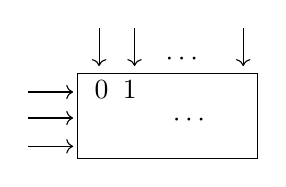
\begin{tikzpicture}[x=0.6cm,y=0.6cm]
\draw (0,0) rectangle (3.8,1.8);
\draw[->] (0.45,2.75)--(0.45,1.95);
\draw[->] (1.2,2.75)--(1.2,1.95);
\draw[->] (3.5,2.75)--(3.5,1.95);
\node at (2.25,2.1) {$\cdots$};
\draw[->] (-1.05,1.4)--(-0.1,1.4);
\draw[->] (-1.05,0.85)--(-0.1,0.85);
\draw[->] (-1.05,0.25)--(-0.1,0.25);
\node at (0.5,1.45) {$0$};
\node at (1.1,1.45) {$1$};
\node at (2.4,0.8) {$\cdots$};
\end{tikzpicture}
\end{adjustbox}
\end{center}
Рассм. $0,1$-матрицы с данными суммами по строкам и столбцам.

Через такие числа всё выражается.

\begin{adjustbox}{max width=\linewidth}
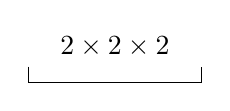
\begin{tikzpicture}[x=1cm,y=1cm]
\node at (1.1,0.3) {$2\times2\times2$};
\draw (0,0.05)--(0,-0.15)--(2.2,-0.15)--(2.2,0.05);
\end{tikzpicture}
\end{adjustbox}

Будет построен комплекс

(3)
\begin{equation*}
0\longrightarrow C_0\overset{d(A)}{\longrightarrow}C_1
\overset{d(A)}{\longrightarrow}\ldots
\overset{d(A)}{\longrightarrow}C_n\longrightarrow0
\end{equation*}
[На правом поле, после двух вертикальных черт:] $d(A)$ линейно зависит от матрицы $A$
\begin{equation*}
A\text{ вырождена}\quad\Longleftrightarrow\quad\text{нарушение точности}
\end{equation*}
Пусть $0\to C_0\to C_1\to\ldots\to C_n\to0$
\begin{equation*}
\operatorname{Det}C_\bullet=
\frac{\Lambda^{\max}C_0\otimes\Lambda^{\max}C_2\otimes\ldots}
{\Lambda^{\max}C_1\otimes\Lambda^{\max}C_3\otimes\ldots}
\end{equation*}
[Зачёркнуто: \Unclear{GELFAND-P001515}{lower-cancelled-wedge}{$\Lambda^{\max}C_1$ или $\Lambda^{\max}C_i$}]
\begin{equation*}
\sum(-1)^i\dim C_i=\sum(-1)^i\dim H_i
\end{equation*}
Из док-ва следует естеств. изоморфизм.
\begin{equation*}
\operatorname{Det}C_\bullet\cong\operatorname{Det}H_\bullet
\end{equation*}
Ацикличность $C_\bullet\Rightarrow\operatorname{Det}H_\bullet=\mathbb C$.

\SourcePage{GELFAND-P001516}{unlabelled}
Выберем базисы во всех $C_i$ $\Rightarrow$ возникает элемент
[зачёркнуто: \Unclear{GELFAND-P001516}{top-cancelled}{в}]
\begin{equation*}
\alpha\in\operatorname{Det} C.
\end{equation*}
и, следовательно, число.

$\alpha$ зависит от $A$ рационально и часто полиномиально.

Для $\det$ $2\times2$ матр. $ad-bc$ получается
\begin{equation*}
0\to\mathbb{C}\to\mathbb{C}^{4}\to\mathbb{C}^{7}\to\mathbb{C}^{4}\to0
\end{equation*}
\begin{center}
\begin{adjustbox}{max width=\linewidth}
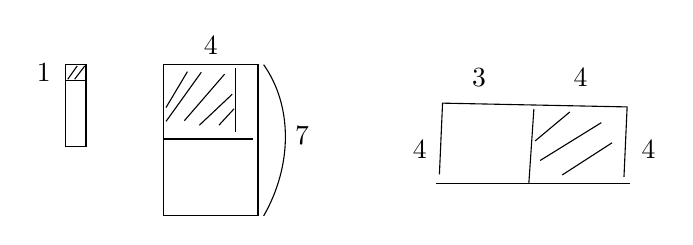
\begin{tikzpicture}[x=0.8cm,y=0.8cm]
\draw (0,1.1) -- (0,2.4) -- (0.32,2.4) -- (0.32,1.1) -- (0,1.1);
\draw (0,2.15) -- (0.32,2.15);
\draw (0.03,2.17) -- (0.18,2.38);
\draw (0.14,2.17) -- (0.30,2.38);
\node at (-0.35,2.27) {$1$};
\draw (1.55,0) -- (3.05,0) -- (3.05,2.4) -- (1.55,2.4) -- (1.55,0);
\draw (1.55,1.22) -- (2.97,1.22);
\draw (2.70,1.33) -- (2.70,2.35);
\draw (1.59,1.72) -- (1.93,2.29);
\draw (1.59,1.50) -- (2.15,2.28);
\draw (1.88,1.51) -- (2.52,2.25);
\draw (2.12,1.44) -- (2.64,1.93);
\draw (2.43,1.44) -- (2.67,1.70);
\draw (3.14,0) .. controls (3.60,0.8) and (3.60,1.75) .. (3.14,2.4);
\node at (2.3,2.70) {$4$};
\node at (3.75,1.28) {$7$};
\draw (5.88,0.52) -- (8.95,0.52);
\draw (5.93,0.66) -- (5.98,1.79) -- (8.91,1.73) -- (8.86,0.62);
\draw (7.35,0.52) -- (7.43,1.70);
\draw (7.45,1.19) -- (8.00,1.65);
\draw (7.53,0.88) -- (8.50,1.48);
\draw (7.88,0.65) -- (8.67,1.16);
\node at (6.56,2.20) {$3$};
\node at (8.17,2.20) {$4$};
\node at (5.62,1.05) {$4$};
\node at (9.25,1.05) {$4$};
\end{tikzpicture}
\end{adjustbox}
\end{center}

\begin{center}
\begin{adjustbox}{max width=\linewidth}
\begin{tikzpicture}[x=0.9cm,y=0.9cm]
\node at (0,0.80) {$ad-bc=$};
\draw (1.65,1.22) -- (1.90,1.22) -- (1.90,1.47) -- (1.65,1.47) -- (1.65,1.22);
\draw (1.66,1.24) -- (1.84,1.46);
\draw (1.74,1.23) -- (1.89,1.42);
\node at (1.78,1.73) {$1$};
\node at (1.40,1.34) {$1$};
\node at (2.26,1.30) {$\cdot$};
\draw (2.70,1.07) -- (3.44,1.07) -- (3.51,1.83) -- (2.77,1.83) -- (2.70,1.07);
\draw (2.74,1.35) -- (3.02,1.76);
\draw (2.84,1.21) -- (3.36,1.62);
\draw (3.08,1.11) -- (3.44,1.43);
\draw (3.28,1.11) -- (3.47,1.28);
\node at (3.13,2.08) {$4$};
\node at (3.77,1.46) {$4$};
\draw (1.34,0.75) -- (4.07,0.75);
\draw (2.08,-0.38) -- (2.84,-0.38) -- (2.89,0.31) -- (2.15,0.31) -- (2.08,-0.38);
\draw (2.10,-0.06) -- (2.45,0.24);
\draw (2.13,-0.29) -- (2.58,0.09);
\draw (2.41,-0.35) -- (2.73,-0.10);
\draw (2.57,-0.34) -- (2.78,-0.20);
\node at (2.50,0.52) {$3$};
\node at (3.22,-0.02) {$3$};
\node at (7.10,0.75) {$\Rightarrow\ \text{степень}=2$};
\end{tikzpicture}
\end{adjustbox}
\end{center}

$\det={}$ Н. О. Д. $\max$ миноров матрицы $4\times7$

\begin{center}— · —\end{center}
\underline{капранов}
\begin{equation*}
X=P(V_1^*)\times\cdots\times P(V_d^*),\qquad O(1)=O(1,\ldots,1)
\end{equation*}
\begin{center}
\begin{adjustbox}{max width=\linewidth}
\begin{tikzcd}[row sep=large,column sep=large]
\text{\Unclear{GELFAND-P001516}{bicomplex-top-left}{$O$}} \arrow[r] \arrow[d]
& \Omega^1(1) \arrow[r,"\partial(A)"] \arrow[d,"\tau(A)"]
& \Omega^2(2) \arrow[r,"\partial(A)"] \arrow[d,"\tau(A)"]
& \cdots \\
O(1) \arrow[r] \arrow[d,"\tau(A)"]
& \Omega^1(2) \arrow[r] \arrow[d,"\tau(A)"]
& \Omega^2(3) \arrow[r] \arrow[d]
& \cdots \\
O(2) \arrow[r] \arrow[d]
& \Omega^1(3) \arrow[r] \arrow[d]
& \Omega^2(4) \arrow[r] \arrow[d]
& \cdots \\
\vdots & \vdots & \vdots &
\end{tikzcd}
\end{adjustbox}
\end{center}
\SourceFigure{GELFAND-P001516}{bicomplex-top-left}{В верхнем левом узле бикомплекса овальный знак $O$ обведён несколькими штрихами; исходная форма под обводкой не вполне различима. Остальные узлы, стрелки и подписи переданы по видимой схеме.}
\SourceFigure{GELFAND-P001516}{bicomplex-vertical-stroke}{У вертикальной стрелки от $\Omega^1(1)$ к $\Omega^1(2)$ с подписью $\tau(A)$ нижний наконечник направлен вниз; у верхнего конца имеется короткий косой штрих влево, похожий на часть верхнего наконечника. Направление вниз уверенно видно; характер верхнего штриха не установлен.}
\begin{align*}
1)\quad &\partial(A)^2=0,\qquad \partial(A)\partial(B)=-\partial(B)\partial(A)\\
2)\quad &\tau(A)\partial(A)=\partial(A)\tau(A)\\
3)\quad &\tau(A)\tau(B)=\tau(B)\tau(A)
\end{align*}

\SourcePage{GELFAND-P001517}{70}
Тогда фиксируем $m\geq0$; получим
\begin{equation*}
C_i^{(m)}\ \text{\Unclear{GELFAND-P001517}{top-isomorphism}{$\cong$}}\quad
\Gamma(X,\Omega^i(i+m))\oplus\Gamma(X,\Omega^{i-1}(i+m))
\end{equation*}
[Справа под формулой:] (свёртка бикомплекса, сост. из 2-х строк)
\begin{equation*}
A\in\Gamma(X,O(1))
\end{equation*}
$\tau(A)$ — умножение на $A\in\Gamma(X,O(1))$

$\partial(A)$ на $\Omega^k(\ell)$
\begin{equation*}
\partial(A)\omega=\frac{1}{\ell+1}A\cdot d\omega+\frac{\ell}{\ell+1}(dA)\cdot\omega
\end{equation*}
\Unclear{GELFAND-P001517}{differential-formula}{Знак $+$ и коэффициенты в формуле $\partial(A)\omega$ переданы буквально.}

\begin{center}— · —\end{center}
\underline{Зелевинский}
\begin{equation*}
X\subset\mathbb{P}(V^*)
\end{equation*}
[Над «лин.»: \Unclear{GELFAND-P001517}{above-lin-mark}{1 или вертикальный штрих}.]

лин. нормально, т.е. $H^0(X,O(1))={}$
[зачёркнуто: \Unclear{GELFAND-P001517}{cancelled-before-v}{неразборчивый знак}] $V$.

\underline{Примеры}

1) $V$ — непривод. представление полупростой группы $G$

$X\subset\mathbb{P}(V^*)$ — проективизация орбиты старшего вектора.

2) Пусть на $V$ действует \Unclear{GELFAND-P001517}{torus-abbreviation}{компл.} тор $(\mathbb{C}^*)^n=H$

Характеры $\mathbb{Z}^n$, в ней выделен набор
\begin{equation*}
\mathbb{Z}^n=((\mathbb{C}^*)^n)^{\wedge}\ni\chi_1,\ldots,\chi_N,\qquad N=\dim V,\quad V=\mathbb{C}^N
\end{equation*}
Все $\chi_j$ лежат на афф. гиперплоскости в $\mathbb{Z}^n$
\begin{equation*}
X=(\text{замык. общей орбиты этого компл. тора})=\overline{H(1,\ldots,1)}
\end{equation*}
\Unclear{GELFAND-P001517}{orbit-overbar}{Над $H(1,\ldots,1)$ проведена горизонтальная черта с наконечникообразными концами.}
Пересеч. примеров 1 и 2 — гипердетерминанты.

\SourcePage{GELFAND-P001518}{73}
Поведение числа Бетти на пр-ве предст. мало изучалось!

Подскоки
числа Бетти —
\Unclear{GELFAND-P001518}{top-secondline-afterdash}{важны}
(\Unclear{GELFAND-P001518}{top-parenthesis-first}{1-х} трив.
\Unclear{GELFAND-P001518}{top-parenthesis-final}{монодр.}!)

\underline{Гипотеза:}
[Зачёркнуто: \Unclear{GELFAND-P001518}{hypothesis-cancel}{неразборчиво}.]
полин. Джонса — лишь
[Зачёркнуто: \Unclear{GELFAND-P001518}{scheme-cancel}{неразборчиво}.]
схема вычисления тех инвариантов,
к-рые раньше надо вычислять.

\medskip
\underline{20/II-89 г.}\qquad \underline{План сем. Вишика}

[Две колонки, разделённые вертикальной чертой. Левая колонка:]
\begin{enumerate}
\item[1.] Фурсиков «\Unclear{GELFAND-P001518}{fursikov-title}{Оптим. упр.}»
\item[2.] Вайнберг
\item[3.] \Unclear{GELFAND-P001518}{kuksin-name}{Куксин}.
\item[4.] Агранович
\end{enumerate}
[Под пунктом 4 зачёркнут отдельный знак:
\Unclear{GELFAND-P001518}{program-left-cancel}{неразборчиво}.]

[Правая колонка:]
\begin{enumerate}
\item[5.] Синай «опер. Шред. с
\Unclear{GELFAND-P001518}{sinai-coefficients}{к.п.} коэфф.»
\item[6.] Бирман или Соломяк
(\Unclear{GELFAND-P001518}{birman-topic}{спектр. ас.} для оп. Шред.)
\item[7.] Бабин, \underline{Вишик}: об аттр. для неогр. обл.
\item[8.] Тужилин «Миним. пов.»
\item[9.] \underline{Гельфанд}, \underline{Захаревич}.
\end{enumerate}

\medskip
\underline{20/II-89}\qquad \underline{Бейлинсон.}

\underline{Люстиг.}

След. объекты примерно эквивалентные
\begin{enumerate}
\item[1.] Представления
[зачёркнуто: \Unclear{GELFAND-P001518}{representations-cancel}{неразборчиво}]
полупростых алг. групп в конечной хар-ке.
\item[2.] Представления квантовых групп при $q=$ корню из 1.
\item[3.] Представления группы петель с целым уровнем.
\item[4.] Геометрия афф. клеток Шуберта
\end{enumerate}

\SourceFigure{GELFAND-P001518}{weight-diagram}{Горизонтальная линия.
Слева над ней подпись «ст. вес.», ниже «разм.».
Над линией слева направо стоят $0$, $1$, $2$, $\ell'$, $p-1$, $\ell$, $2p-1$.
Вертикальные короткие штрихи отмечены под $0$, $p-1$ и $2p-1$.
Под $0$ написано $1$; перед этой единицей выше расположен зачёркнутый неразборчивый знак.
Под $p-1$ стоит $p$, под $2p-1$ — $2p$.
Ниже линии проведена дуга от области $\ell'$ к области $\ell$;
у обоих верхних концов видны сходящиеся штрихи, похожие на стрелки к линии,
но правый конец особенно бледен.}

$X_\ell$ — неприв. предст. со старшим весом $\ell$

$V_\ell$ — предст. в однор. многочленах.

Пусть $\ell$ — целое число, тогда
\begin{equation*}
0\to X_{\ell'}\to V_\ell\to X_\ell\to 0
\end{equation*}

\medskip
\underline{И.М. Гельфанд.}

Рассм. 6 прямых на
проект. плоскости

\SourceFigure{GELFAND-P001518}{line-arrangement}{Слева внизу рисунок пересекающихся линий.
Видны почти горизонтальная линия, линия сверху слева вниз направо,
линия снизу слева вверх направо, более крутая толстая линия снизу вверх с небольшими изломами,
а также тонкая, местами прерывистая крутая линия.
Пересечения показаны без буквенных подписей; часть тонких штрихов плохо различима.
Справа от рисунка расположен текстовый блок из трёх строк, переданных ниже.
Справа от этих строк проведена вертикальная черта, под ними — горизонтальная;
от нижней черты направлена стрелка вниз к «Док-во:».}

[Под рисунком:]
(\Unclear{GELFAND-P001518}{infinity-caption}{и} беск. удал.)

[Справа от рисунка:]

5 прямых\newline
Всегда\newline
6 огр. областей

[Правее:]
Это возникает в интеграле
\begin{equation*}
\int\frac{dx}{\sqrt{(x-a)(x-b)(x-c)(x-d)}}
\end{equation*}

[Под стрелкой:]
\underline{Док-во:} рассм.
\Unclear{GELFAND-P001518}{proof-phrase}{пуч. из} прямых.

\SourcePage{GELFAND-P001519}{unlabelled}
\underline{Капранов}

\underline{$X$ — пов. $K3$, если}
\begin{enumerate}
\item[1)] $\pi_1(X)=0$
\item[2)] $\Omega_X^2$ тривиально (как голом. расслоение)
\end{enumerate}
[Под $\Omega_X^2$ вписано: «(рассл. форм объёма)».]

(т.е. $\exists$ голом. форма объёма
[зачёркнуто: \Unclear{GELFAND-P001519}{volume-cancel}{неразборчиво}],
нигде не обр. в 0)

Они все гомеом. и даже диффеом.

\underline{Пример:} 2-мерн. компл. тор
\begin{gather*}
T=\mathbb{C}^2/\mathbb{Z}^4\\
\downarrow
\end{gather*}
\begin{center}
\Unclear{GELFAND-P001519}{kummer-quotient}{$T/(2x=0)$}
\qquad ($x$ и $-x$ отожд.)
\end{center}

Возник. 16 особ. точек; (пов. Куммера)

Гладкая будет после разрешения особенностей.

\begin{center}
\begin{adjustbox}{max width=\linewidth}
\begin{tikzpicture}
\draw (-1,0) -- (-0.1,0);
\draw (0.2,0.1) -- (1.1,0.1);
\draw (0.06,-0.02) -- (0.06,0.08);
\end{tikzpicture}
\end{adjustbox}
\end{center}

\begin{equation*}
G(2,4)\subset\mathbb{P}^5\qquad\text{(квадрика)}
\end{equation*}

\begin{center}
\begin{adjustbox}{max width=\linewidth}
\begin{tikzpicture}
\node (q) at (0,0) {$Q$};
\node[anchor=west] at (0.3,0) {$\cap G(2,4)=F$};
\node[anchor=west] (quadric) at (-0.25,-0.9) {квадрика};
\draw[->] (0,-0.3) -- (0,-0.65);
\end{tikzpicture}
\end{adjustbox}
\end{center}



\end{document}
